\documentclass[../../book-main.tex]{subfiles}
\usepackage[UTF8]{ctex}
\graphicspath{{\subfix{../..}}}

\begin{document}

\chapter{学习线性和独立结构}
\label{ch:classic}\label{ch:linear-independent}

\begin{quote}
\hfill  ``{\em 做数学的艺术在于找到那个包含所有普遍性的特殊案例}.''

$~$\hfill -- 大卫·希尔伯特
\end{quote}
\vspace{5mm}

% \DP{第1节:PCA(确定性),PPCA(统计性),矩阵补全/RPCA(两者)。添加幂迭代等。}

% \DP{第2节:正交字典学习(确定性),伯努利-高斯ODL(统计性),允许不同类型的误差 \(\implies\) ICA(统计性)。添加幂迭代(来自 \href{https://openreview.net/pdf?id=SJeY-1BKDS}{西蒙的论文})。}

% \DP{第3节:过完备基上的稀疏编码(确定性)。快速稀疏编码算法如ISTA。如果你给我基,那就是稀疏恢复,否则你必须学习基(例如KSVD)}
% \yima{实际上,约翰的团队有一系列关于学习过完备字典的工作,具有强正确性和理论保证。}

% \DP{写一个历史注释,说明这些变体与中心问题的关系}

%\DP{在第3章中,注意扩散泛化PCA(使用彭的论文)作为在所有级别上学习去噪器}

\textit{真实数据具有低维结构。} 为了说明这一点,让我们考虑一个简单的例子:当卫星不工作时,电视上的静态。在每个帧(大约每 \(\frac{1}{30}\) 秒),屏幕大小为 \(H \times W\) 的 RGB 静态,大致是从 \([0, 1]^{3 \times H \times W}\) 上的均匀分布中独立采样的。理论上,静态 \textit{可能} 在任何给定帧上解析为自然图像,但即使你花一千年来观察电视屏幕,它也不会。这种差异可以用以下事实来解释:\(H \times W\) 自然图像的集合在超立方体 \([0, 1]^{3 \times H \times W}\) 中占据了一个微不足道的小部分。特别是,它是低维的。类似的现象也发生在所有其他类型的自然数据中,如文本、音频和视频。因此,当我们设计系统和方法来处理自然数据并学习其结构或分布时,这是自然数据的一个中心属性,我们需要考虑。 %\sdb{我们是否需要这个例子?我们已经有了 \ref{sec:intro-low-dimensionality}} \DP{我觉得重新强调一下是好的,它将连接那些跳过介绍的读者。此外,这个例子更倾向于图像和视频,这将激发本书后半部分的内容。}

因此,我们的中心任务是学习一个在高维空间中具有低内在维度的分布。在本节的剩余部分,我们将讨论几种 \textit{经典} 方法来执行此任务,针对分布的几种较为 {\em 理想化} 的模型,即几何上线性或统计上独立的模型。虽然这些模型和方法本身很重要且有用,但我们在这里讨论它们,因为它们激发、启发并作为更现代方法的前身或类比,这些方法适用于更一般的分布,涉及深度(表示)学习。

我们的主要方法可以概括为:
\begin{tcolorbox}
    \textit{给定一个或多个来自数据分布的真实样本的(有噪声或不完整的)观测值,获得该样本的估计。}
\end{tcolorbox}
这一方法支撑了几个经典的数据处理方法,我们在本章中讨论这些方法。
\begin{itemize}
    \item 第 \ref{sec:lowrank} 节 --- 主成分分析(PCA):给定来自一个低维子空间上的分布的有噪声样本,获得位于该子空间上的真实样本的估计。
    \item 第 \ref{sec:ica} 节 --- 完全字典学习和独立成分分析(ICA):给定来自几个低维子空间的并集(\textit{不是}张成空间)上的分布的有噪声样本,获得真实样本的估计。
    \item 第 \ref{sec:dictionary_learning} 节 --- 稀疏编码和过完备字典学习:给定来自一个由几个不相干向量组合支持的分布的有噪声样本,例如坐标轴,获得具有相同性质的真实样本的估计。
\end{itemize}
正如我们将在后续章节中揭示的,在深度学习时代,现代方法本质上也采用了相同的方法来学习。

在本章中,如上所述,我们做出简化建模假设,这些假设本质上假设数据具有几何上(几乎,分段)线性结构和统计上独立的成分。在第 \ref{ch:intro} 章中,我们已经将这种数据模型称为“解析模型”。这些建模假设使我们能够推导出具有可证明的效率保证\footnote{在数据和计算复杂性方面。}的高效算法,用于大规模数据处理。然而,它们对于通常复杂的现实世界数据分布来说是不完美的模型,因此它们的基本假设仅近似成立。这意味着这些算法的详细分析所提供的保证在实际数据情况下也仅近似成立。尽管如此,本章中讨论的技术本身是有用的,而且不仅如此,它们还作为“具有普遍性的特例”,即它们为更一般的(深度)学习范式提供了指导性的动机和直觉,这些范式处理更一般的数据分布。% \sdb{感觉需要更多的冒险性和权威性(更多地依赖于真正好的开场引用来支持)...也许还可以更清楚地说明每个部分的结构?(也可以与第1章的“解析模型”部分联系起来)}\DP{尝试了一下}

% \yima{为了与后续章节保持一致,我们可以将所有模型和问题统一到相同的压缩自编码框架中:
% \begin{equation}
% \x \xrightarrow{\hspace{2mm} \mathcal{E} \hspace{2mm}}  \z \xrightarrow{\hspace{2mm} \mathcal{D} \hspace{2mm}}   \hat{\x}.    
% \end{equation}
% 我会非正式地说,本章是针对理想化的分布,这些分布允许编码器 $\mathcal{E}$ 或解码器 $\mathcal{D}$ 是{\em 浅层和线性}的。对于另一个相反的方向,可以通过高效的(优化)算法来实现。我甚至会进一步具体说明每个模型和问题,明确相关的编码和解码算法是什么。 
% }

% \yima{伙计们,再次强调,本章的目的不是介绍这些问题本身。我们的目标是展示它们如何从同一视角和共同的计算框架中统一起来,这与未来章节的内容也是一致的。}

% \sdb{我们应该根据 Yi 的先前评论重写这一介绍/动机部分,以帮助聚焦后续的展示。然后相应地重写和精简 PCA 部分。我现在正在重写第 2.2 节。}

%wacwwwwwwwwwwwwwwwwwwwdadw本章连接了数据分析的经典根源与低维结构:几何上线性、统计上独立。

%外在/内在?表示?

%在后续中回响的三(?)件事:
%\begin{enumerate}
%    \item \textbf{我们对现实有什么假设?}我们的模型;数学建模。
%    \item \textbf{我们如何用模型进行计算?}简单模型 $\implies$
%        高效计算。
%    \item \textbf{它有效吗?}当模型假设成立 $\implies$ 数学证明
%        它有效。(当它“可以”时 $\implies$ 有界“有效”)。
%\end{enumerate}
%即使模型过于理想化,其解也可能传达适用于更一般情况的基本思想。

%\section{低维结构和分布建模}
\pw{第56页和第65页缺少一些图}

\section{低维子空间} \label{sec:lowrank}

\subsection{主成分分析(PCA)} \label{sub:pca}

对于低维结构可能的最简单建模假设是所谓的\textit{低秩}假设。设 \(D\) 为数据空间的维度,我们假设我们的数据属于一个低维子空间,维度为 \(d \ll D\),可能加上一些小扰动。这最终成为了一些复杂数据的几乎有效的假设,例如手写数字图像、人脸数据 \cite{BasriR2003-PAMI} 和运动数据 \cite{Vidal-GPCA},然而,正如我们将看到的,它将非常有利于全面分析。

\begin{figure}
    \centering
    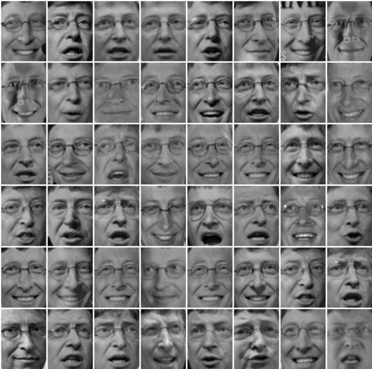
\includegraphics[width=0.3\linewidth]{figs_chap2/faces.png}
    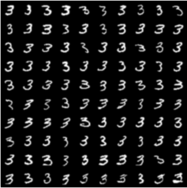
\includegraphics[width=0.295\linewidth]{figs_chap2/handwritten-digits.png}
    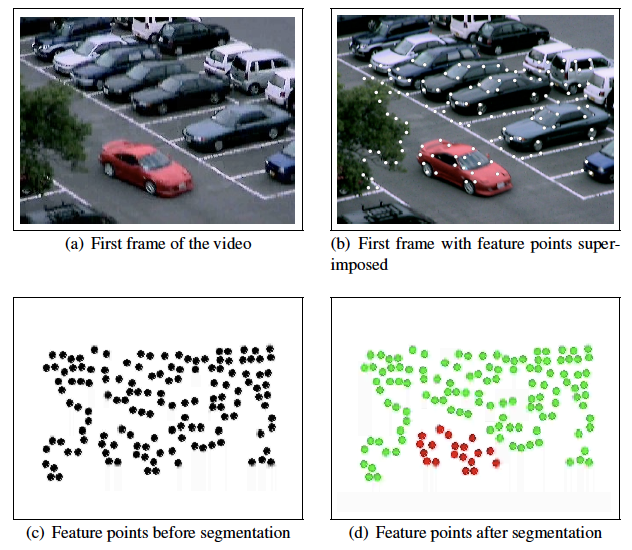
\includegraphics[width=0.35\linewidth]{figs_chap2/motion.png}    
    \caption{人类面孔、手写数字和移动物体上的特征图像。尽管它们的外观似乎有很大的差异,但每组数据都跨越了一个非常低维的(几乎线性)子空间。}
    \label{fig:enter-label}
\end{figure}

\paragraph{问题表述。}
为了用数学符号表示这一点,我们用一个正交矩阵 \(\vU \in \O(D, d) \subseteq \R^{D \times d}\) 表示一个子空间 \(\cS \subseteq \R^{D}\),维度为 \(d\),使得 \(\vU\) 的列张成 \(\cS\)。然后,我们说我们的数据 \(\{\vx_{i}\}_{i = 1}^{N} \subseteq \R^{D}\) 具有(近似)低秩结构,当且仅当存在一个正交矩阵 \(\vU_{o} \in \O(D, d)\),向量 \(\{\vz_{o, i}\}_{i = 1}^{N} \subseteq \R^{d}\),以及\textit{小}向量 \(\{\veps_{i}\}_{i = 1}^{N} \subseteq \R^{D}\),使得
\begin{equation}\label{eq:pca_dgp}
    \vx_{i} = \vU_{o}\vz_{o, i} + \veps_{i}, \qquad \forall i \in [N].
\end{equation}
这里 \(\veps_{i}\) 是扰动,使数据偏离完美低秩;我们模型中的这些扰动的存在允许我们量化在偏离模型的情况下分析仍然相关的程度。因此,为了从这些数据中处理所有信息,这相当于恢复 \(\vU_{o}\),也称为\textit{主成分}。幸运的是,这是一个计算上可行的任务,称为主成分分析,我们现在讨论如何解决它。

给定数据 \(\{\vx_{i}\}_{i = 1}^{N}\) 分布如 \eqref{eq:pca_dgp},我们旨在恢复模型 \(\vU_{o}\)。一个自然的方法是找到子空间 \(\vU_{\star}\) 和潜在向量 \(\{\vz_{\star, i}\}_{i = 1}^{N}\),它们最接近于获得 \(\vx_{i} \approx \vU_{\star}\vz_{\star, i}\)。也就是说,我们旨在解决以下问题
\begin{equation}\label{eq:pca_sparse_recovery_problem}
    \min_{\vU, \{\vz_{i}\}_{i = 1}^{N}}\frac{1}{N}\sum_{i = 1}^{N}\norm{\vx_{i} - \vU\vz_{i}}_{2}^{2}.
\end{equation}

\paragraph{通过去噪进行子空间编码-解码。}
为了简化这个问题,对于固定的 \(\vU\),我们有(证明作为练习):
\begin{align*}
    \min_{\{\vz_{i}\}_{i = 1}^{N}}\frac{1}{N}\sum_{i = 1}^{N}\norm{\vx_{i} - \vU\vz_{i}}_{2}^{2} 
    &= \frac{1}{N}\sum_{i = 1}^{N}\min_{\vz_{i}}\norm{\vx_{i} - \vU\vz_{i}}_{2}^{2} \\
    &= \frac{1}{N}\sum_{i = 1}^{N}\norm{\vx_{i} - \vU\vU^{\top}\vx_{i}}_{2}^{2}. 
\end{align*}
也就是说,\(\vz_i = \vU^\top\vx_i\) 是上述最小化问题的最优解。

现在,我们可以将原始的优化问题写成关于 \(\vU\) 和 \(\{\vz_{i}\}_{i = 1}^{N}\) 的形式,即
\begin{equation}\label{eq:pca_equals_denoising}
    \min_{\vU, \{\vz_{i}\}_{i = 1}^{N}}\frac{1}{N}\sum_{i = 1}^{N}\norm{\vx_{i} - \vU\vz_{i}}_{2}^{2} = \min_{\vU}\frac{1}{N}\sum_{i = 1}^{N}\norm{\vx_{i} - \vU\vU^{\top}\vx_{i}}_{2}^{2}.
\end{equation}
注意,等式 \eqref{eq:pca_equals_denoising} 右侧的问题是一个 \textit{去噪} 问题:给定低秩数据的噪声观测 \(\vx_{i}\),我们旨在找到 \(\vx_{i}\) 的 \textit{无噪声} 副本,记为 $\hat{\vx}_i$。也就是说,$\hat{\vx}_i = \vU\vU^\top \vx_i$。注意,这是子空间中距离 $\vx_i$ 最近的点。通过求解等价问题,即找到最佳子空间,参数化为基 \(\vU\),\textit{去噪器} 是投影矩阵 \(\vU\vU^{\top}\),它将噪声数据点 $\x_i$ 投影到子空间上。%去噪是高维数据分析的基本构建块之一,我们将在本书中多次讨论它,因为我们将讨论的许多算法本质上是对特定数据模型(如 \eqref{eq:pca_dgp},但更复杂)的去噪。

将上述过程结合起来,我们本质上得到了一个简单的编码-解码方案,将数据点 $\vx$ 从 $\R^D$ 映射到低维(潜在)空间 $\R^d$,然后再映射回 $\R^D$:
\begin{equation}
\x \xrightarrow{\hspace{2mm} \mathcal{E} = \vU^\top \hspace{2mm}}  \z \xrightarrow{\hspace{2mm} \mathcal{D} = \vU \hspace{2mm}}   \hat{\x}.  
\label{eqn:autoencoding-PCA}
\end{equation}
这里 $\vz \in \R^d$ 可以被视为数据点  $\x \in \R^D$ 的紧凑编码(或潜在表示),而学习到的子空间基 $\vU$ 作为相应的码本,其列是(学习到的)最优码字。该过程通过将 $\x$ 投影到由 $\vU$ 跨越的子空间上来实现对 $\x$ 的去噪功能。

\paragraph{计算子空间基。}
现在,我们继续计算。设 \(\vX = \mat{\vx_{1}, \dots, \vx_{N}} \in \R^{D \times N}\) 是列向量为观测值 \(\vx_{i}\) 的矩阵。我们有(证明作为练习)
\begin{align}
    \argmin_{\vU}\frac{1}{N}\sum_{i = 1}^{N}\norm{\vx_{i} - \vU\vU^{\top}\vx_{i}}_{2}^{2}
    &= \argmax_{\vU}\frac{1}{N}\sum_{i = 1}^{N}\norm{\vU^{\top}\vx_{i}}_{F}^{2} \\ 
    &= \argmax_{\vU}\tr\rc{\vU^{\top}\bp{\frac{\vX\vX^{\top}}{N}}\vU}.
\end{align}
因此,为了计算主成分,我们找到使 \(\tr(\vU^{\top}(\vX\vX^{\top}/N)\vU)\) 最大的正交矩阵 \(\vU\)。事实上,最佳的矩阵 \(\vU^{\star}\) 的列是 \(\vX\vX^{\top}/N\) 的 \textit{前 \(d\) 个特征向量}。虽然可以通过暴力计算获得,例如归纳证明,但我们在这里不这样做;相反,我们通过考虑 \(d = 1\) 的情况来提供一些直觉。然后,我们只需要恢复一个单位向量 \(\vu\),并求解问题 \(\max_{\vu} \vu^{\top}(\vX\vX^{\top}/N)\vu\)。这是 \(\vX\vX^{\top}/N\) 的所谓 \textit{瑞利商},该问题的最优解是 \(\vX\vX^{\top}/N\) 的最大特征值对应的特征向量。因此,\(d = 1\) 情况下的解对应于我们对一般 \(d\) 情况的提议解。总之,我们有
\begin{tcolorbox}
    \textit{主成分对应于最优线性去噪器,由 \(\vX\vX^{\top}/N\) 的前 \(d\) 个特征向量给出。}
\end{tcolorbox}

\begin{remark}
    在某些数据分析任务中,数据矩阵 \(\vX\) 的格式使得每个数据点是 \textit{行} 而不是 \textit{列},如这里所示。在这种情况下,主成分是 \(\vX^{\top}\vX\) 的前 \(d\) 个特征向量。
\end{remark}

\begin{remark}[Basis Selection via Denoising Eigenvalues]
    在许多情况下,要么我们的数据不会真正遵循子空间加噪声模型,要么我们不知道子空间的真实潜在维度 \(d\)。在这种情况下,我们必须选择 \(d\);这个问题被称为 \textit{模型选择}。在 PCA 的受限情况下,一种进行模型选择的方法是计算 \(\vX\vX^{\top}/N\) 并寻找相邻特征值从大到小变化的实例;这是特征值较大的索引是“真实维度 \(d\)”的一个指标,而 \(\vX\vX^{\top}/N\) 的其余特征值是由噪声或扰动 \(\veps_{i}\) 贡献的。模型选择是一个困难的问题,如今在深度学习时代,它被称为“超参数优化”,通常通过暴力搜索或贝叶斯优化来完成。%\sdb{通过“阈值化噪声”来学习 $\vU$}
\end{remark}

\begin{remark}[去噪样本]
    \eqref{eq:pca_equals_denoising} 右侧的表达式,即
    \begin{equation}\label{eq:orthogonal_denoising}
        \min_{\vU}\frac{1}{N}\sum_{i = 1}^{N}\norm{\vx_{i} - \vU\vU^{\top}\vx_{i}}_{2}^{2},
    \end{equation}
    是一个已知的 \textit{去噪问题},之所以这样命名,是因为它是一个优化问题,其解 \textit{去除了样本中的噪声,使其符合子空间}。去噪——学习一个映射,从有噪声的样本中去除噪声,使其符合数据结构(如 \eqref{eq:pca_dgp},但可能更复杂)——是学习分布的一种常见方法,将在后续章节和整篇论文中讨论。
\end{remark}

\begin{remark}[神经网络解释]
    如果我们进行 PCA,我们近似恢复了由参数 \(\vU_{\star}\) 编码的分布的支持。学习的去噪映射然后具有形式 \(\vU_{\star}\vU_{\star}^{\top}\)。除了是一个去噪器之外,这可以被视为一个 \textit{简单的两层权重绑定线性神经网络}:第一层乘以 \(\vU_{\star}^{\top}\),第二层乘以 \(\vU_{\star}\),即
    \begin{equation}
        \operatorname{denoise}(\vx) = \underbrace{\vU_{\star} \circ \underbrace{\id \circ \underbrace{\vU_{\star}^{\top}\vx}_{\text{第一层}}}_{\text{第一层的后激活}}}_{\text{“NN”的输出}}
    \end{equation}
    与标准的两层神经网络相比,我们看到了结构上的相似性:
    \begin{equation}
        \operatorname{NN}(\vx) = \underbrace{\vW_{\star} \circ \underbrace{\mathrm{ReLU} \circ \underbrace{\vU_{\star}^{\top}\vx}_{\text{第一层}}}_{\text{第一层的后激活}}}_{\text{NN 的输出}}
    \end{equation}
    特别地,PCA 可以解释为 \textit{学习一个简单的两层去噪自编码器},这是最简单的非平凡神经网络之一。在这个框架中,\textit{学习的表示}只是 \(\vU_{\star}^{\top}\vx\)。通过这种方式,PCA 作为深度表示学习的一个模型问题,我们将在本论文中进一步探讨。请注意,在这个类比中,表示反映了或投影了输入数据到学习的低维结构。这个性质在将来将特别相关。
\end{remark}

\begin{exercise}
    证明,对于任何对称矩阵 \(\vA\),问题 \(\max_{\vU \in \O(D, d)}\tr\left(\vU^{\top}\vA\vU\right)\) 的解是矩阵 \(\vU^{\star}\),其列是 \(\vA\) 的前 \(d\) 个单位特征向量。
\end{exercise}

\subsection{通过幂迭代追求低秩结构}

有一种计算上高效的方法来估计 \(\vX\vX^{\top}/N\) 的前几个特征向量,或者任何对称半正定矩阵 \(\vM\),称为 \textit{幂迭代}。这种方法是我们在本章后面讨论的几种高维数据分析算法方法的构建块,因此我们在这里讨论它。

现在,设 \(\vM\) 是一个对称半正定矩阵,存在一个由 \(\vM\) 的特征向量 \((\vw_{i})_{i = 1}^{D}\) 组成的 \(\R^{D}\) 的标准正交基,对应的特征值为 \(\lambda_{1} \geq \cdots \geq \lambda_{D} \geq 0\)。根据定义,任何特征向量 \(\vw_i\) 满足 \(\lambda_i \vw_i = \vM \vw_i\)。因此,对于任何 \(\lambda_i > 0\),\(\vw_i\) 是以下方程的一个“不动点”:
\begin{equation}
    \vw = \frac{\vM\vw}{\norm{\vM\vw}_{2}}.
    \label{eqn:PCA-fixed-point}
\end{equation}
然后,我们可以使用以下迭代来计算不动点:
\begin{equation}\label{eq:power_iteration}
    \vv_{0} \sim \dNorm(\vzero, \vone), \qquad \vv_{t + 1} \gets \frac{\vM\vv_{t}}{\norm{\vM\vv_{t}}_{2}}.
\end{equation}
在极限情况下,\(\vv_{t}\) 将收敛到 \(\vM\) 的一个最大单位范数特征向量。

为什么这样的迭代会起作用?首先,注意对于所有 \(t\),我们有
\begin{equation}
    \vv_{t} = \frac{\vM\vv_{t - 1}}{\norm{\vM\vv_{t - 1}}_{2}} = \frac{\vM^{2}\vv_{t - 2}}{\norm{\vM\vv_{t - 1}}_{2}\norm{\vM\vv_{t - 2}}_{2}} = \cdots = \frac{\vM^{t}\vv_{0}}{\prod_{s = 1}^{t}\norm{\vM\vv_{s}}_{2}}.
\end{equation}
因此,\(\vv_{t}\) 与 \(\vM^{t}\vv_{0}\) 的方向相同,并且是单位范数,因此我们可以写
\begin{equation}
    \vv_{t} = \frac{\vM^{t}\vv_{0}}{\norm{\vM^{t}\vv_{0}}_{2}}.
\end{equation}

因为 \(\vM\) 的所有特征向量 \(\vw_{i}\) 构成了 \(\R^{D}\) 的一个标准正交基,我们可以写
\begin{equation}
    \vv_{0} = \sum_{i = 1}^{D}\alpha_{i}\vw_{i},
\end{equation}
其中,因为 \(\vv_{0}\) 是高斯分布的,所以 \(\alpha_{i}\) 都是非零的,概率为 \(1\)。因此,我们可以使用我们之前对 \(\vv_{t}\) 的表达式来写
\begin{equation}
    \vv_{t} = \frac{\vM^{t}\vv_{0}}{\norm{\vM^{t}\vv_{0}}_{2}} = \frac{\sum_{i = 1}^{D}\lambda_{i}^{t}\alpha_{i}\vw_{i}}{\norm{\sum_{i = 1}^{D}\lambda_{i}^{t}\alpha_{i}\vw_{i}}_{2}} = \frac{\sum_{i = 1}^{D}\lambda_{i}^{t}\alpha_{i}\vw_{i}}{\sum_{i = 1}^{D}\lambda_{i}^{t}\abs{\alpha_{i}}}. 
\end{equation}
现在,让我们考虑 \(\lambda_{1} > \lambda_{2} \geq \cdots \geq \lambda_{D} \geq 0\) 的情况。(重复的最大特征值的情况类似。)那么我们可以写
\begin{equation}
    \vv_{t} = \frac{\alpha_{1}\vw_{1} + \sum_{i = 2}^{D}(\lambda_{i}/\lambda_{1})^{t}\alpha_{i}\vw_{i}}{\abs{\alpha_{1}} + \sum_{i = 2}^{D}(\lambda_{i}/\lambda_{1})^{t}\abs{\alpha_{i}}}.
\end{equation}
因为 \(\lambda_{1} > \lambda_{i}\) 对于所有 \(i > 1\),求和项中的项以指数速度趋近于 \(0\),剩下的极限是
\begin{equation}
    \lim_{t \to \infty}\vv_{t} = \frac{\alpha_{1}}{\abs{\alpha_{1}}}\vw_{1} = \sign(\alpha_{1})\vw_{1},
\end{equation}
这是 \(\vM\) 的一个最大单位特征向量。 \(\vM\) 的最大特征值 \(\lambda_{1}\) 可以通过 \(\vv_{t}^{\top}\vM\vv_{t}\) 来估计,这同样迅速地收敛到 \(\lambda_{1}\)。

为了找到第二个最大特征向量,我们将幂迭代算法应用于 \(\vM - \lambda_{1}\vv_{1}\vv_{1}^{\top}\),该矩阵的特征向量为 \((\vw_{i})_{i = 2}^{D}\),对应的特征值为 \((\lambda_{i})_{i = 2}^{D}\)。通过重复这个过程 \(d\) 次,我们可以非常高效地估计 \(\vM\) 的前 \(d\) 个特征向量,对于任何对称半正定矩阵 \(\vM\) 都是如此。因此,我们也可以将其应用于 \(\vX\vX^{\top}/N\) 来恢复前 \(d\) 个主成分,这是我们最初的目标。注意,这种方法一次恢复一个主成分;我们将在后续章节中将其与其他算法方法进行对比,例如全局目标函数的梯度下降。

% \DP{备注:局部迭代方法获取成分与下一节(及以后)优化全局模型:有历史根源和算法见解...}

% 我们在第 \ref{sec:power_iteration} 节中讨论它。 \sdb{我们真的想把计算推迟到最后吗?(我同意这是一个很好的结束注释;我想知道我们是否可以为每个示例讨论计算,然后在最后提供统一的解释/理解?(这可以作为本章的前瞻结论))}

\subsection{概率主成分分析}

请注意,上述公式对数据生成过程没有做出任何统计假设。然而,通常会在给定的数据模型中包含统计元素,因为这可能会为分析结果提供进一步的启发性解释。因此,我们提出一个自然的问题:\textit{低维结构的统计类比是什么?}我们的答案是,一个低维的\textit{分布}是指其支撑集中在低维几何结构上的分布。

为了说明这一点,我们讨论\textit{概率主成分分析(PPCA)}。这种表述可以被视为常规PCA的统计变体。数学上,我们现在将数据视为从一个取值于\(\R^{D}\)的随机变量\(\vx\)中抽取的样本(有时也称为\textit{随机向量})。我们说\(\vx\)具有(近似)低秩统计结构,当且仅当存在一个正交矩阵\(\vU_{o} \in \O(D, d)\),一个取值于\(\R^{d}\)的随机变量\(\vz_{o}\),以及一个\textit{小}的随机变量\(\veps\)取值于\(\R^{D}\),使得\(\vz_{o}\)和\(\veps\)相互独立,并且
\begin{equation}
    \vx = \vU_{o}\vz_{o} + \veps.
\end{equation}
我们的目标仍然是恢复\(\vU_{o}\)。为此,我们设置与子节\eqref{sub:pca}中类似的问题,即在子空间\(\vU\)和随机变量\(\vz\)上进行优化,以解决以下问题:
\begin{equation}
    \min_{\vU, \vz}\Ex\norm{\vx - \vU\vz}_{2}^{2}.
\end{equation}
由于我们正在寻找最佳的随机变量\(\vz\),我们可以为每个\(\vx\)的值分别找到其实现\(\vz(\vx)\)。进行与子节\eqref{sub:pca}中相同的计算,我们得到 %\sdb{这里的符号有点奇怪(期望中有一个\(\vz(\vx)\)?并且\(\vz\)被重用了?)}
\begin{equation}\label{eq:ppca_denoising}
    \min_{\vU, \vz}\Ex\norm{\vx - \vU\vz}_{2}^{2} = \min_{\vU}\Ex\min_{\vz(\vx)}\norm{\vx - \vU\vz(\vx)}_{2}^{2} = \min_{\vU}\Ex\norm{\vx - \vU\vU^{\top}\vx}_{2}^{2},
\end{equation}
再次强调,估计的子空间与主成分\(\vU\)对应的去噪器\(\vU\vU^{\top}\)将数据投影到该子空间上。与之前一样,我们得到
\begin{align}
    \argmin_{\vU}\Ex\norm{\vx - \vU\vU^{\top}\vx}_{2}^{2} 
    &= \argmax_{\vU}\Ex\norm{\vU^{\top}\vx}_{2}^{2} \\
    &= \argmax_{\vU}\tr(\vU^{\top}\Ex[\vx\vx^{\top}]\vU),
\end{align}
后一个问题的解就是二阶矩矩阵\(\Ex[\vx\vx^{\top}]\)的前\(d\)个主成分。实际上,上述问题与前一子节中计算主成分的方程在视觉上非常相似,只是用\(\Ex[\vx\vx^{\top}]\)替换了\(\vX\vX^{\top}/N\)。事实上,后者是前者的估计量。两种表述实际上做了同样的事情,具有相同的实际解决方案——计算数据矩阵\(\vX\)的左奇异向量,或者等价地计算估计的协方差矩阵\(\vX\vX^{\top}/N\)的前\(d\)个特征向量。然而,统计表述具有额外的解释。假设\(\Ex[\vz_{o}] = \vzero\)和\(\Ex[\veps] = \vzero\),我们有
\begin{equation}
    \Ex[\vx] = \vU_{o}\Ex[\vz_{o}] + \Ex[\veps] = \vzero,
\end{equation}
因此\(\Cov[\vx] = \Ex[\vx\vx^{\top}]\)。现在计算\(\Cov[\vx]\),我们有
\begin{equation}
    \Cov[\vx] = \vU_{o}\Cov[\vz_{o}]\vU_{o}^{\top} + \Cov[\veps] = \vU_{o}\Ex[\vx\vx^{\top}]\vU_{o}^{\top} + \Cov[\veps].
\end{equation}
特别是,如果\(\Cov[\veps]\)很小,那么\(\Cov[\vx] = \Ex[\vx\vx^{\top}]\)近似为一个低秩矩阵,具体来说是秩\(d\)。因此,\(\Ex[\vx\vx^{\top}]\)的前\(d\)个特征向量基本上概括了整个协方差矩阵。但它们也是主成分,因此我们可以将主成分分析解释为对\(\Cov[\vx]\)进行低秩分解。

\begin{remark}
    通过使用PCA的概率观点,我们能够更清晰、更定量地理解它与去噪之间的关系。首先,考虑\eqref{eq:ppca_denoising}中的去噪问题,即
    \begin{equation}
        \min_{\vU}\Ex\norm{\vx - \vU\vU^{\top}\vx}_{2}^{2}.
    \end{equation}
    不难证明,如果\(\veps\)是一个各向同性的高斯随机变量,即分布为\(\veps \sim \dNorm(\vzero, \sigma^{2}\vI)\),\footnote{只要它们支持\(\R^{D}\)的所有部分,其他分布也可以工作,但高斯分布在这里是最容易处理的。}那么对于这个问题的任何解\(\vU_{\star}\),我们有
    \begin{equation}
        \vU_{\star}\vU_{\star}^{\top} = \vU_{o}\vU_{o}^{\top}
    \end{equation}
    因此,真实的支撑子空间,即\(\cS_{o} \doteq \Range(\vU_{o})\),可以通过\(\vU_{\star}\)的列的张成来恢复,因为
    \begin{equation}
        \cS_{o} = \Range(\vU_{o}) = \Range(\vU_{o}\vU_{o}^{\top}) = \Range(\vU_{\star}\vU_{\star}^{\top}) = \Range(\vU_{\star}).
    \end{equation}
    特别地,学习到的去噪映射\(\vU_{\star}\vU_{\star}^{\top}\)是到\(\cS_{o}\)的正交投影,将噪声点推到真实的支撑子空间上。在只有有限样本的情况下,我们也可以建立类似的理论结果,如子节\ref{sub:pca}所述,但这需要更多的努力和技术细节。%\DP{包括正式的错误率吗?}
\end{remark}

% \sdb{也许可以更多地讨论去噪连接的概念意义(纠正错误...与模型选择和基于分数的生成建模的联系...样本复杂度和概念上的见解)。也许可以为\(\vz\)高斯的情况进行这些讨论?(ICA章节是“非高斯的”)}

% 本节中的其他例子将类似地进行。我们将介绍一个动机例子,并给出问题的几何和统计形式化。

\subsection{矩阵补全}

%\DP{TODO: 插入与深度学习的联系;这个过渡不太好...}
%\yaodong{为什么把矩阵补全放在这里?}
在前几个子节中,我们讨论了学习低秩几何或统计分布的问题,其中数据是从具有加性噪声的子空间中采样的。但这不是唯一值得研究的低维分布扰动类型。在本子节中,我们将介绍一类非加性误差,这类误差在深度学习中变得越来越重要。让我们考虑一个情况,其中我们有一些数据\(\{\vx_{i}\}_{i = 1}^{n}\)根据\eqref{eq:pca_dgp}生成。现在我们将它们排列成一个矩阵\(\vX = \mat{\vx_{1}, \dots, \vx_{N}} \in \R^{D \times N}\)。与之前不同,我们不直接观察\(\vX\);相反,我们假设我们的观察在传输过程中被破坏,我们得到了
\begin{equation}
    \vY = \vM \odot \vX,
\end{equation}
其中\(\vM \in \{0, 1\}^{D \times N}\)是一个已知的\textit{掩码},\(\odot\)是逐元素乘法。在这种情况下,我们的目标是仅根据被破坏的观察\(\vY\)、掩码\(\vM\)和\(\vX\)是(近似)低秩的知识来恢复\(\vX\)(从这一点开始,我们可以使用PCA来恢复\(\vU_{o}\)等)。这被称为\textit{低秩矩阵补全}。

有许多优秀的资源讨论了解决这个问题的算法和方法 \cite{Wright-Ma-2022}。确实,这个问题及其类似的低秩结构恢复问题的推广,可以通过“鲁棒主成分分析”来解决。我们在这里不会详细讨论解决方案方法。相反,我们将讨论在什么条件下这个问题是\textit{合理的}可以解决的。一方面,在最荒谬的情况下,假设矩阵\(\vX\)的每个条目都是独立于其他条目选择的。那么,即使只有一个条目缺失,我们有\(DN - 1\)个条目,也无法精确恢复\(\vX\)。另一方面,假设我们知道\(\vX\)的秩恰好为1,这是一个对数据低维结构的极其强的条件,我们正在处理的掩码是
\begin{equation}
    \vM = \mat{\vone_{(D - 1) \times 1} & \vzero_{(D - 1) \times (N - 1)} \\ 1 & \vone_{1 \times (N - 1)} }.
\end{equation}
那么我们知道数据分布在一条直线上,我们还知道这条直线上的一个向量——它只是矩阵\(\vY = \vM \odot \vX\)的第一列。从每列的最后一个坐标,掩码也向我们揭示了这一点,我们可以求解每列,因为对于每个最终坐标,直线上只有一个具有该坐标的向量。因此,我们可以完美地重建\(\vX\),并且只需要线性数量的观测值\(D + N - 1\)。

在现实世界中,实际问题介于上述两个极端情况之间。然而,这两个极端之间的差异,以及之前关于主成分分析的讨论,揭示了一个普遍的真理核心:
\begin{tcolorbox}
    \textit{数据分布的低维性和结构化程度越高,处理起来就越容易,需要的观测值就越少——前提是算法有效地利用了这种低维结构。}
\end{tcolorbox}
也许可以预料到,我们将在这个手稿的剩余部分中反复遇到这个主题,从下一节开始。

% 解决这个问题的一个初步想法是建立一个优化问题,其中候选解在所有未屏蔽的索引处与观测值匹配,并且具有近似低秩。这个想法可以通过以下问题形式化表达:
% \begin{equation}
%     \min_{\substack{\vW \\ \vY = \vM \odot \vW}}\rank(\vW).
% \end{equation}
% 然而,这个形式化存在两个问题:
% \begin{enumerate}
%     \item \(\rank\) 函数既不连续也不凸,因此直接优化是计算上不可行的。
%     \item 这个形式化可能没有正确处理近似低秩变量,这些变量表面上是高秩的,但实际上只是低秩加上噪声。
% \end{enumerate}
% 为了解决第一个问题,我们使用所谓的秩函数的 \textit{凸松弛},即核范数 \(\norm{\cdot}_{*}\),定义为 
% \begin{equation}
%     \norm{\vA}_{*} = \tr([\vA^{\top}\vA]^{1/2})
% \end{equation}
% 其中 \(\vB^{1/2}\) 是正半定平方根。核范数的三个关键性质是(1)它是凸函数,(2)它形成了秩函数的包络,即 \(\norm{\vA}_{*} \leq \rank(\vA)\) 对所有 \(\vA\) 成立,提供了一个有效的下界,可以有效地优化,(3)它也是高效的计算。这三个性质使其成为在矩阵补全问题中替代秩函数的有吸引力的替代品。因此,我们使用以下问题来恢复 \(\vX\):
% \begin{equation}
%     \min_{\substack{\vW \\ \vY = \vM \odot \vW}}\norm{\vW}_{*}.
% \end{equation}
% 最后,为了处理第二个问题,我们使用该问题的拉格朗日形式,得到 
% \begin{equation}
%     \min_{\vW}\bc{\frac{1}{2}\norm{\vY - \vM \odot \vW}_{F}^{2} + \lambda \norm{\vW}_{*}}.
% \end{equation}
% 这个形式化具有吸引人的数学性质,以及前面讨论的概念基础。
% \sdb{这一节感觉不太合适...也许我们可以在这里讨论一下“通过低维结构纠正粗大误差(缺失数据)”的想法,通过一个关于低秩矩阵补全不是无望的基本概念讨论,然后在后面讨论压缩感知时再回到这个问题?}

% \sdb{还要注意,一般矩阵补全之所以非平凡,是因为模型选择比小噪声 PCA/去噪要困难得多...我们目前在 PCA 部分没有讨论模型选择。如果你把模型选择部分去掉,问题可能变得足够简单,可以在这里具体地写出来}

% \DP{如果我们知道损坏,可以使用 PCA 或矩阵补全;如果不知道,可以使用鲁棒 PCA。一段话。}

% \begin{itemize}
%     \item 古典例子:随机噪声 \(\neq\) 相干图像 \(\implies\) 相干图像具有某种严重的结构
%     \item 如何捕捉这种结构?
%     \item 图像的正确数据结构?序列?(如果我们能证明这些是子空间,那就太好了,否则就推到后面)
%     \item 愚蠢地:支持在我们所知道的最简单的低维对象上(子空间 \(\implies\) PCA)
%     \item 不那么愚蠢地:由某个易于描述的过程生成(稀疏编码、字典学习、低秩矩阵补全)
%     \item 更不愚蠢地:属于一个通用流形
%     \item 数据有时是从某个分布中抽取的
%     \item 最简单的低维高斯分布对应于子空间情况
%     \item 不那么简单的:伯努利-高斯自然对应于字典学习,高斯瘦矩阵的外积对应于低秩矩阵
%     \item 通用的低维概率分布可以用流形很好地近似
%     \item 本节其余部分:如何在这些(最简单、不那么简单、一般)假设下学习——经典方法
% \end{itemize}

% \DP{本小节的主要目标:连接数据的几何和统计结构;讨论数据在高层次上的结构(低秩或低维流形);高斯/高斯混合假设,近似}

% \subsection{通过去噪学习线性子空间} 
% 使用学习单个线性子空间的经典案例来说明通过压缩(降维)从噪声样本中学习低维模型的一般方法。介绍幂迭代算法...

% 可能还应该联系最近的扩散视角:当扩散-去噪过程专门用于低秩高斯时,它等价于经典的PCA。此外,关于所需样本数量的特征化。

% \subsection{通过补全和纠错学习}
% 可能值得提及变体,如矩阵补全、鲁棒PCA,用于在更一般的“噪声”或“扰动”概念下学习低维线性模型。

\section{完全低维子空间的混合}% 和完全字典学习 } 
\label{sec:ica}
正如我们所见,低秩信号模型足够丰富,可以提供数据中的低维性和表示和恢复错误的高效和可扩展计算算法之间的相互作用的完整图景。 
这些模型隐含了一个 \textit{线性} 和对称的自编码管道 \eqref{eqn:autoencoding-PCA}: 
\begin{equation*}
    \vz = \cE(\vx) = \vU^\top \vx, \quad \hat{\vx} = \cD(\vz) = \vU \vz,
\end{equation*}
这可以从有限的 $\vx$ 样本中通过主成分分析(例如,使用幂方法高效求解)来证明学习,只要 $\vx$ 的分布确实是线性的。
这是一个限制性的假设——正如 20 世纪杰出的统计学家哈罗德·霍特林(Harold Hotelling)\footnote{巧合的是,他也因对主成分分析的发展和命名做出贡献而闻名 \cite{Hotelling1933}。} 在乔治·丹齐格(George Dantzig)首次介绍线性规划理论时提出异议 \cite{Dantzig2002-eh},
\begin{quote}
\centering
    \textit{“...我们都知道世界是非线性的。”}
\end{quote}

即使考虑到其优雅和简洁,低秩假设也过于严格,无法广泛应用于建模现实世界的数据。一个关键的限制是假设一个单一的线性子空间负责生成结构化的观测值。在许多实际应用中,由不同低维子空间的混合生成的结构提供了一个更强大和现实的模型。例如,考虑一个视频序列,捕捉多个不同对象的运动,每个对象都受到其独立的位移(图\ref{}a)\pw{添加图片}。在对个体运动做出适当假设的情况下,每个对象在视频帧的拼接序列中负责一个独立的低维子空间\cite{VidalR2004-ECCV}。另一个例子是通过学习一个模型来建模自然图像的分布,该模型描述了图像中像素的\textit{块}(空间上连续的像素集合)的分布(图\ref{}b)\pw{添加图片}。与我们之前看到的Eigenface示例不同,在Eigenface示例中,具有匹配姿势的人脸图像可以用一个单一的低维子空间很好地近似,自然图像中特定位置的块可以对应于具有非常不同属性的对象——例如,由于遮挡边界而具有不同的颜色或形状。因此,用一个单一的子空间建模块的分布是徒劳的,但子空间的混合在实践中表现得非常好(图\ref{}c)\pw{添加图片}。\footnote{我们将在第\ref{ch:representation}章中回到这一观察,我们将展示它可以被显著推广,以生成适用于大规模现代数据集的强大表示。}

\begin{figure}
    \centering
    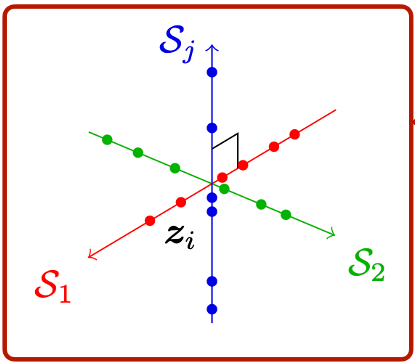
\includegraphics[width=0.35\linewidth]{chapters/subspaces.png}
    \caption{在低维子空间的混合上的数据,例如$\mathcal{S}_j = \mbox{span}(\vU_j)$。}
    \label{fig:subspaces}
\end{figure}

在本节中,我们将开始讨论当数据分布具有由\textit{低维子空间的混合}建模的结构时,压缩自编码的概念和算法基础,如图\ref{fig:subspaces}所示。在这种情况下,解码器映射将几乎与单个子空间的情况一样简单:我们简单地表示为
\begin{equation}\label{eq:mixture-subspaces-decoder-first-cut}
    \hat{\x} = \cD(\vz) = \left( \sum_{k=1}^K \pi_k(\vz)\vU_k \right) \vz,
\end{equation}
其中$\pi_k : \R^d \to \set{0,1}$是一组\textit{稀疏}的权重随机变量,使得在求和中仅选择一个子空间$\mathcal{S}_k = \mbox{span}(\vU_k)$。
然而,将此类数据$\vx$编码为合适的表示$\vz$,并从数据中学习这样的编码器-解码器对,将证明更加复杂。

我们将看到,来自\textit{稀疏表示}和\textit{独立成分分析}的丰富文献中的思想如何通过稀疏性的视角,自然地重新表述上述解码器架构,相应的编码器架构(通过类似于主成分分析的幂方法算法获得),以及从数据中学习此类编码器-解码器对的正确性和效率的强大保证。从这个意义上说,混合线性低维结构的情况已经导致了我们在本书中将更广泛地发展的表示学习的关键组成部分。

%\subsection{表示子空间的混合:稀疏字典}
\subsection{稀疏使用的正交字典}

%\yima{不确定为什么先介绍这个模型,而不是ICA?} \sdb{根据之前的反馈,我想将这一部分从“非高斯性”中移开,因为“非高斯性”是ICA的动机,而更多地转向稀疏性和几何结构。我将在这一部分之后介绍ICA,但仅通过BG假设,认为这是通过稀疏性的视角来激发的。然后,算法可以像上一稿那样引入,但不需要所有抽象的峰度动机。老实说,ICA的经典动机方式在我看来并不完全符合全局表示学习的主题(ICA的动机是:我们假设独立的成分;考虑到可识别性,这意味着我们只能恢复非高斯成分;我们优化峰度以尝试找到非高斯成分)——这就是为什么我从这个模型开始。此外,子空间混合(或高斯混合)在技术上似乎将在本书中发挥更重要的作用。}

设$\vU_1, \dots, \vU_K$,每个大小为$D \times d$,表示$\R^D$中$K$个维度为$d$的子空间的正交基。
从几何上讲,说$\vx$遵循由$\vU_1, \dots, \vU_K$参数化的子空间混合分布意味着
\begin{equation}\label{eq:mixture-of-subspaces-geometric}
    \vx = \vU_k \vz  \quad \text{for some} \enspace k \in [K],\enspace \vz \in \R^d.
\end{equation}
正如我们在PCA和线性结构的情况下所看到的,这种几何模型的统计类比是$\vx$遵循一个\textit{高斯混合}分布:即,
\begin{equation}\label{eq:mixture-of-subspaces-statistical}
    \vx \sim \sum_{k=1}^K \pi_k \cN(\mathbf{0}, \vU_k\vU_k^\top), \quad \text{for some} \enspace \pi_k \geq 0,\enspace \sum_{k=1}^K \pi_k = 1.
\end{equation}
换句话说,对于每个$k \in [K]$,$\vx$在低维子空间$\Span(\vU_k)$上是高斯分布的,概率为$\pi_k$。
尽管模型\eqref{eq:mixture-of-subspaces-statistical}看起来很简单,但它已经足够丰富,可以作为表示学习理论的基础,该理论可以扩展到大规模的现代数据集。
然而,我们得等到第\ref{ch:representation}章,才能发展出这一理论的先决条件。

\begin{remark}[高斯混合与高斯叠加]
应该注意的是,上述模型\eqref{eq:mixture-of-subspaces-statistical}是一个高斯分布的混合,不应与通过叠加的高斯变量的混合相混淆,例如
\begin{equation}
    \vx = \sum_{i=1}^n w_i \vx_i, \quad \vx_i \sim \cN(\mathbf{0}, \vU_i\vU_i^\top),
\end{equation}
其中$\vx_i$是独立的随机高斯向量,$w_i$是一组固定的权重。根据高斯向量的性质,这样的叠加$\vx$仍然是一个高斯分布。
\end{remark}

目前,我们关注的是由\eqref{eq:mixture-of-subspaces-geometric}提供的几何视角。
有一个在代数上更方便的替代条件表示。考虑一个\textit{提升}表示向量$\vz = [\vz_1^\top, \dots, \vz_K^\top]^\top \in \R^{dK}$,使得$\vz$是\textit{$d$-稀疏}的,其支撑在$dK$个坐标中的$K$个连续不重叠的块之一上。
然后,\eqref{eq:mixture-of-subspaces-geometric}可以等价地写为
\begin{equation}\label{eq:mixture-of-subspaces-dictionary-pre}
    \vx = 
    \underbrace{
    \begin{bmatrix} 
    | & \hdots & |  \\
    \vU_1 & \hdots & \vU_K  \\
    | & \hdots & | 
    \end{bmatrix} 
    }_{\vU}
    \underbrace{
    \begin{bmatrix} \vz_1 \\ \vdots \\ \vz_K \end{bmatrix}
    }_{\vz},
    \quad
    \norm*{
    \begin{bmatrix} \norm*{\vz_1}_2 \\ \vdots \\ \norm*{\vz_K}_2 \end{bmatrix}
    }_0 = 1.
\end{equation}
这里,$\ell^0$“范数”$\norm{\,\cdot\,}_0$通过计数非零项的数量来衡量稀疏性:
\begin{equation}\label{eq:ell-zero-norm}
    \norm{\vz}_0 = \abs*{\set{i \given z_i \neq 0}},
\end{equation}
矩阵$\vU \in \R^{D \times Kd}$称为一个\textit{字典},其中所有$\{\vU_i\}_{i=1}^K$都是码字。通常,如果混合中的子空间数量$K$足够大,字典$\vU$中的列数没有上限。在$Kd < D$的情况下,$\vU$称为\textit{欠完备};
当$Kd = D$时,称为\textit{完备};当$Kd > D$时,称为\textit{过完备}。

现在,\eqref{eq:mixture-of-subspaces-dictionary-pre}建议了一个方便的放松,以使分析变得可行:而不是将$\vx$建模为来自$K$个\textit{特定}子空间$\vU_1, \dots, \vU_K$的混合,我们也可以从一个字典$\vU \in \R^{D \times m}$开始,其中$m$可能小于或大于$D$,并简单地寻求用稀疏性$\norm{\vz}_0$足够小的$\vx = \vU \vz$来表示。
这导致了$\vx$的\textit{稀疏字典模型}:
\begin{equation}\label{eq:mixture-of-subspaces-dictionary}
    \vx =  \vU \vz + \veps,
    \quad
    \norm{\vz}_0 \ll d,
\end{equation}
其中$\veps$表示一个未知的噪声向量。
几何上,这意味着$\vx$接近于$\vU$的$\norm{\vz}_0$列的子集的张成空间,
这使得它成为混合子空间模型\eqref{eq:mixture-of-subspaces-geometric}的一个实例,其中$K$的值非常大,并且子空间$\vU_k$之间存在特定的相关性。
%然而,人们发现这种放松在简单的实际任务中是有用的,并且它具有丰富的概念和算法理论,我们将在本章的剩余部分中进行阐述。

%\subsection{学习稀疏使用的正交字典}

\paragraph{稀疏编码的正交字典。}
现在我们可以制定本节将研究的低维子空间混合的压缩自编码问题。
我们假设我们有来自未知稀疏字典模型 \eqref{eq:mixture-of-subspaces-dictionary} 的样本 $\vX = [\vx_1, \dots \vx_N]$,可能添加了噪声 $\veps_i$。
让我们从假设稀疏字典模型 \eqref{eq:mixture-of-subspaces-dictionary} 中的字典 $\vU$ 是完整且正交的开始,\footnote{正如我们很快会看到的,对于完整的情况,我们通过假设正交性不会失去任何一般性。} 并且每个系数向量 $\vz$ 是 $d$-稀疏的,其中 $d \ll D$。
此外,不失一般性地假设 $\vU$ 是一个正交矩阵(练习 \ref{exercise:whitening})。
在这种情况下,压缩自编码等同于 \textit{正确学习正交字典 $\vU$}:我们可以取 $\cE(\vx) = \vU^T \vx$ 作为编码器和 $\cD(\vz) = \vU \vz$ 作为解码器,并且 $\cD = \cE^{-1}$。
我们的任务是:
\begin{tcolorbox}
    假设 $\vx$ 满足具有正交字典 $\vU$ 和稀疏度 $d$ 的稀疏字典模型 \eqref{eq:mixture-of-subspaces-dictionary}。
    给定足够多的 $\vx$ 的样本 $\vX = [\vx_1, \dots, \vx_N]$,
    通过某种优化过程 \textit{学习字典 $\vU$},使得
    $\cE(\vx) = \vU^\top \vx$ 和 $\cD(\vz) = \vU \vz$ 在 $\vx$ 上形成无损自编码对。
\begin{equation}
\x \xrightarrow{\hspace{2mm} \mathcal{E} = \vU^\top \hspace{2mm}}  \z \xrightarrow{\hspace{2mm} \mathcal{D} = \vU \hspace{2mm}}   \hat{\x}.  
\label{eqn:autoencoding-DL}
\end{equation}    
\end{tcolorbox}
我们看到,完整字典学习的自编码对 $(\cE, \cD)$ 是对称的,就像单一线性子空间的情况一样,使得编码和解码的计算任务与线性情况一样简单。另一方面,学习字典 $\vU$ 的任务比通过 PCA 学习单一线性子空间严格更困难。
为什么我们不能简单地使用 PCA 来正确学习正交字典 $\vU$,请注意,导致 PCA 的损失函数,即 \eqref{eq:pca_equals_denoising},对矩阵 $\vU$ 的行的旋转完全不变:也就是说,如果 $\vQ$ 是任何 $d \times d$ 正交矩阵,则 $\vU$ 和 $\vU \vQ$ 都是可行的,并且对于 \eqref{eq:pca_equals_denoising} 具有相同的损失。稀疏字典模型在这样的变换下明显不是不变的:如果我们用 $\vU \vQ$ 替换 $\vU$ 并对表示系数 $\vz$ 进行相应的旋转 $\vQ^\top \vz$,我们将破坏 $\vz$ 的稀疏结构,违反建模假设。因此,我们需要开发新的算法来学习正交字典。

\subsection{完整字典学习}
\label{sec:complete-dictionary}
%\sdb{需要在这里强调低维性的作用。目前,低维性 $\iff$ 在这个模型中的稀疏性;这里只有表面联系}

在本节中,我们将推导用于解决正交字典学习问题的算法。更具体地说,我们假设观测向量 $\vx \in \R^D$ 遵循统计模型
\begin{equation}
    \vx = \vU_o \vz + \veps, 
    \label{eq:ica-model-ch2}
\end{equation}
其中 $\vU_o \in \R^{D \times D}$ 是未知的正交字典,$\vz$ 是具有统计独立分量 $z_i$ 的随机向量,每个分量均值为零,$\veps \in \R^D$ 是独立的小(高斯)噪声随机向量。目标是从 $\vx$ 的样本中恢复 $\vU_o$(从而恢复 $\vz$)。
%模型 \eqref{eq:ica-model-ch2} 在盲源分离等应用中出现,其中每个独立分量 $z_i$ 表示一个独立的源(例如,音乐录音中与不同乐器相关的声音),这些源叠加产生观测 $\vx$。
%它也是通过子空间混合模型从高维数据中提取特征的基本原语,我们很快就会看到。

这里我们假设每个独立分量 $z_i$ 的分布为 $$z_i \sim \mathrm{Bern}(\theta) \cdot \cN(0, 1/\theta).$$ 即它是伯努利随机变量与概率为 $\theta$ 时取值为 $1$,概率为 $1-\theta$ 时取值为 $0$ 的乘积,以及一个独立的方差为 $1/\theta$ 的高斯随机变量。这种分布形式正式被称为 {\em 伯努利-高斯} 分布。 
归一化选择使得 $\Var(z_i) = 1$,从而 $\bE[\norm{\vz}_2^2]=d$。 
%利用独立性和标准高斯分布的四阶矩为 $3$ 的事实,可以计算出 $\kurt(z_i) = 3\theta(1-\theta) > 0$,因此该模型确实适用于独立成分分析。
这种建模假设意味着独立分量向量 $\vz$ 通常是高度稀疏的: 
我们计算 $\bE\left[\norm{\vz}_0\right] = d\theta$,当 $\theta$ 与 $d$ 成反比时,这个值很小。

\begin{remark}[正交假设] 
乍一看,假设字典 $\bm U_o$ 是正交的可能看起来有些限制。但实际上并没有损失一般性。可以考虑一个完整的字典为任何可逆的方阵 $\vD$。对于从该字典生成的样本:$\vX = \vD \vZ \in \mathbb{R}^{D\times N}$,很容易证明\footnote{参见例如 \cite{sun2017completeI}},通过数据矩阵 $\vX$ 的预处理: 
\begin{equation}
    \bar{\vX} = \Big(\frac{1}{N\theta} \vX\vX^\top\Big)^{-\frac{1}{2}}\vX,
\end{equation}
则存在一个正交矩阵 $\vD_o \in \mathrm{O}(D)$ 使得
\begin{equation}
    \bar{\vX} = \vU_o\vZ.
\end{equation}
\end{remark}

\begin{figure}
    \centering
    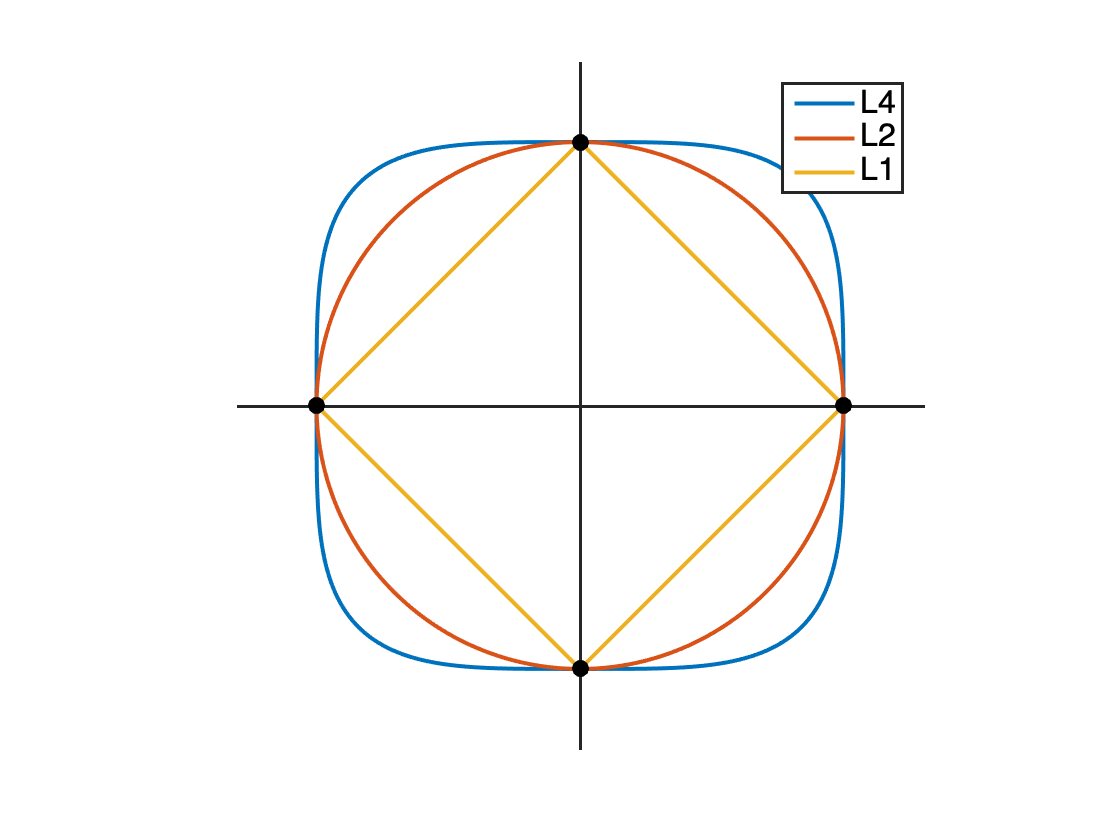
\includegraphics[width=0.6\linewidth]{figs_chap2/2DL4Sphere.png}
    \caption{最大化 $\ell^4$ 范数或最小化 $\ell^1$ 范数可以促进稀疏性(对于球面上的向量)。}
    \label{fig:L4-sphere}
\end{figure}

\paragraph{通过 MSP 算法进行字典学习。}

现在假设我们有一组观测值:
\begin{equation}
    \x_i = \vU_o \vz_i + \veps_i,\ \forall i =1, 2, \ldots, N.
\end{equation}
令 $\vX = [\x_1, \x_2, \ldots, \x_N]$ 和 $\vZ = [\vz_1, \vz_2, \ldots, \vz_N]$。目标是从数据 $\vX$ 中恢复 $\vU_o$。因此,给定任何正交矩阵 $\vA \in \mathrm{O}(D)$,$$\vA\vx_i = \vA\vU_o \vz_i + \vA\veps_i$$ 如果 $\vA = \vU_o^T$(根据假设,噪声 $\veps_i$ 的幅度很小),则该向量几乎是稀疏的。

此外,给定 $\vU_o$ 是正交的且噪声 $\veps$ 很小,向量 $\vx$ 是(几乎)常数 $\bE[\norm{\vx}_2^2] \approx \bE[\norm{\vz}_2^2]=d$。已知对于球面上的向量,最大化 $\ell^4$ 范数等价于最小化 $\ell^0$ 范数(以促进稀疏性),
\begin{equation*}
            \argmax_{\vz \in \mathbb{S}^n}\|\vz\|_{4}\quad\Leftrightarrow\quad \argmin_{\vz \in \mathbb{S}^n}\|\vz\|_{0}.
\end{equation*}
这在图 \ref{fig:L4-sphere} 中有所说明。

对于正交矩阵 $\vA$,它保持 2-范数不变:$\|\vA \x\|_2^2 = \|\x\|_2^2$ 是几乎常数的。因此,为了从 $\vX$ 中找到正确的正交字典 $\vU_o$,我们可以尝试求解以下优化问题:
\begin{equation}\label{eq:orthogonal-dictionary-learning-l4}
    \max_{\vA \in \mathrm{O}(D)}\,
     \frac{1}{4} \norm*{
    \vA \vX
    }_4^4 =  \frac{1}{4} \sum_{i=1}^N \norm*{
    \vA \vx_i
    }_4^4
\end{equation}
这被称为 $\ell^4$ 最大化问题 \cite{Zhai-2020}。
\begin{remark}
    同样已知的是,对于球面上的向量,最小化 $\ell^1$ 范数等价于最小化 $\ell^0$ 范数(以促进稀疏性),
\begin{equation*}
            \argmin_{\vz \in \mathbb{S}^n}\|\vz\|_{1}\quad\Leftrightarrow\quad \argmin_{\vz \in \mathbb{S}^n}\|\vz\|_{0},
\end{equation*}
这也在图 \ref{fig:L4-sphere} 中有所说明。这一事实也可以被利用来有效地和高效地学习字典 $\vA$。实际上,这比这里使用的 $\ell^4$ 范数更早被探索。感兴趣的读者可以参考 \cite{qu2020findingsparsestvectorssubspace} 的工作。
\end{remark}

请注意,上述问题等价于以下约束优化问题:
\begin{equation}\label{eq:orthogonal-dictionary-learning-l4}
    \min\,
    -   \frac{1}{4} \norm*{
    \vA \vX
    }_4^4 \quad \mbox{subject to} \quad  \vA^\top\vA = \vI.
\end{equation}
如 \cite{Wright-Ma-2022} 所示,使用拉格朗日乘数法,可以推导出该问题的最优解应满足以下“不动点”条件:
$$
\vA = \mathcal{P}_{\mathrm O(D)}[( {\vA \vX})^{\circ3}\vX^\top],
$$
其中 $\mathcal{P}_{\mathrm O(D)}[\,\cdot\,]$ 是正交矩阵空间 $\mathrm O(D)$ 上的投影。\footnote{对于任何具有 SVD 的矩阵:$\vM = \vU\bm \Sigma \vV^\top$,$\mathcal{P}_{\mathrm O(D)}[\vM] = \vU \vV^\top$。我们将其留给读者作为练习。}

为了计算上述方程的不动点,类似于我们为 PCA \eqref{eqn:PCA-fixed-point} 计算特征向量,我们可以采取以下幂迭代:
\begin{equation}
    \vA_{t+1} = \mathcal{P}_{\mathrm O(D)}[( {\vA_t \vX})^{\circ3}\vX^\top].
\end{equation}
这被称为由 \cite{Zhai-2020} 提出的“匹配、拉伸和投影”(MSP)算法。已经证明,在广泛条件下,这种贪婪算法确实以超线性速率收敛到正确的解。

\begin{remark}[全局最优性]
约束 $\ell^4$ 最大化问题是一个非凸规划问题。一般来说,人们应该期望任何贪婪(例如梯度下降类型)算法都会收敛到全局最优解。令人惊讶的是,可以证明,与一般的非凸规划不同,$\ell^4$ 最大化在球面上的景观非常良性:所有局部最小值都接近全局最优值,所有临界点都是具有负曲率方向的鞍点。因此,任何能够逃离严格鞍点的下降方法都能证明找到全局最优解。对于更精确的陈述,感兴趣的读者可以参考 \cite{Qu2020Geometric}。
\end{remark}

\begin{remark}[稳定的深度线性网络]
上述计算字典的迭代过程具有自然的增量“深度学习”解释。我们定义 $\delta \vA_{t+1} = \vA_{t+1}\vA_{t}^\top$ 和 $\vZ_t = \vA_t \vX$,则很容易证明
$$\delta \vA_{t+1} = \mathcal{P}_{\mathrm O(D)}[(\vZ_t)^{\circ3} \vZ_t^\top].$$
如果 $\vA_t$ 收敛到正确的字典 $\vD_o$,则上述迭代编码过程本质上等同于一个“深度线性网络”:
$$\vZ \; \longleftarrow \; \vZ_{t+1} =  \underbrace{\delta \vA_{t+1} \delta \vA_{t} \ldots \delta \vA_{1}}_{\color{red} \text{前向构建层}} \vX.$$
请注意,每层的增量变换 $\delta \vA_{t+1}$ 的计算仅依赖于前一层的特征输出 $\vZ_t$。该网络自然稳定,因为每层都是保持范数的正交变换。尽管它类似于线性深度网络,但学习每层不需要反向传播。所有层都在一次前向传递中学习!
\end{remark}

% 我们现在通过一个类似于推导FastICA的方法来推导这个目标的快速不动点算法。
% 与之前一样,我们从正交群上的优化的一阶最优条件开始(练习 \ref{exercise:orthogonal-group-calculus}),对于峰度最大化目标,该条件为
% \begin{equation}\label{eq:l4-ogrp-fxp-step1}
%     \vX \left( \vX \adj \vU \right)^{\hada 3} = \vU \underbrace{\left. \left(
%     \vU\adj \vX \left( \vX \adj \vU \right)^{\hada 3} 
%     + 
%     \left( \vU\adj \vX \right)^{\hada 3} \vX\adj \vU
%     \right) \right/ 2}_{\vS},
% \end{equation}
% 其中对称矩阵 $\vS$ 的值由约束 $\vU\adj \vU = \vI$ 确定。
% 接下来,我们回忆一下,方程 \eqref{eq:l4-ogrp-fxp-step1} 由 $\ell^4$ 最大化问题的 \textit{任何} 临界点满足,而我们寻求一个仅由其最大化点满足的方程。
% 实际上,可以证明,在 \eqref{eq:orthogonal-dictionary-learning-l4} 的任何全局最大化点 $\vU$ 处,出现在 \eqref{eq:l4-ogrp-fxp-step1} 中的矩阵 $\vS$ 实际上是半正定的,即 $\vS \succeq \mathbf{0}$(练习 \ref{exercise:l4-global-maximizers-ogrp})。利用练习 \ref{exercise:orthogonal-group-calculus} 的第 3 部分的结果和奇异值分解,可以很容易地证明,对 \eqref{eq:l4-ogrp-fxp-step1} 的两边进行 \textit{归一化} 可以得到以下不动点表达式,该表达式在 \eqref{eq:orthogonal-dictionary-learning-l4} 的每个局部最大化点处都成立:
% \begin{equation}\label{eq:l4-ogrp-fxp}
%     \mathrm{proj}_{\O(d)}\left(
%     \vX \left( \vX \adj \vU \right)^{\hada 3} 
%     \right)
%     = \vU,
% \end{equation}
% 其中我们回忆一下,$\mathrm{proj}_{\O(d)}(\vX) = \vV \vW\adj$,其中 $\vX = \vV \vS \vW\adj$ 是 $\vX$ 的奇异值分解(练习 \ref{exercise:orthogonal-group-calculus} 的第 3 部分)。
% 迭代由这个不动点表达式的左边定义的映射,可以得到以下通过 $\ell^4$ 最大化进行完整字典学习的幂法,称为 \textit{MSP 算法} \cite{Zhai2019-oc}:
% \begin{equation}
% \begin{split}\label{eq:msp}
%    \vR^+ &= \vX (\vX\adj \vU)^{\hada 3},  \\
%    \vU^+ &= \vV \vW \adj, \quad \text{其中} \enspace \vR^+ = \vV \vS \vW\adj \enspace \textit{是一个 SVD}。
%    \end{split}
% \end{equation}
% 与之前看到的 FastICA 算法一样,MSP 算法在实践中非常快速地收敛到真正的正交字典 $\vU$,除了对称性之外。
% % 具体来说,由于底层目标 \eqref{eq:orthogonal-dictionary-learning-lasso} 的结构,只能恢复 $\vU$ 的行和列的符号置换。
% % 这可以看作是我们的建模假设的结果:无论是伯努利-高斯 ICA 建模假设还是稀疏使用的字典假设(参见练习 \ref{exercise:symmetry-identifiability})。
% 在理想条件下,Zhai 等人证明 MSP 算法 \eqref{eq:msp} 获得了局部收敛的三次速率,与 FastICA 算法的性能相匹配 \cite{Zhai2019-oc}。
% % 同时,它在单轮优化中恢复了整个字典(或 ICA 上下文中的混合矩阵),同时所需的计算操作不比奇异值分解更昂贵,因此在实践中更受欢迎。
% 将字典恢复问题表述为 $\ell^4$ 损失,如公式 \eqref{eq:orthogonal-dictionary-learning-l4} 所示,还具有使数据矩阵中的误差和异常值具有鲁棒性的优势,如 Zhai 等人所证明的 \cite{Zhai-2020}。

% \sdb{添加一个算法框。可能添加一个数值实验。}

%重要的是要认识到,这个目标并不总是能够实现:例如,如果独立分量 $\vz$ 是高斯分布的,即 $\vz \sim \cN(\Zero, \sigma^2\vI)$,
%那么对于任何旋转矩阵 $\vQ$(使得 $\vQ\adj \vQ = \vI$),$\vQ \vz$ 的分布与 $\vz$ 的分布相同(练习),这意味着无法从 $\vx$(或 $\vU$)中重构 $\vz$。
%这种情况被称为(统计)非唯一性;ICA 只有在没有超过一个高斯分量时才是唯一的。
%%即使在添加了这个统计假设后,也请注意无法从 $\vx$ 中估计独立分量的符号或能量 $\Var(z_i)$。
%%因此,我们将假设每个独立分量满足 $\Var(z_i)=1$ 以方便起见,这使得独立分量在符号上是唯一的 \cite{Hyvrinen-2000}。
%这些问题可以通过纯粹的几何概念——\textit{对称性}——来理解:我们在下面的练习 \ref{exercise:symmetry-identifiability} 中探讨了这个问题。
%
%
%将 ICA 的目标与 PCA \eqref{eq:pca_model} 的目标进行对比,其中我们只是寻求用系数 $\vz$ 来 \textit{表示} 数据分布 $\vx$,使得
%$\vx \approx \vU \vz$。几何上,这对应于学习 \textit{子空间} $\mathrm{col}(\vU)$,而不是特定的基 $\vU$ 本身。
%在 ICA 中,我们的任务是精确地学习特定的混合矩阵 $\vU$,或者等价地学习独立分量 $\vz$。
%重要的是要认识到,这个目标并不总是能够实现:例如,如果独立系数 $\vz$ 是高斯分布的,即 $\vz \sim \cN(\Zero, \sigma^2\vI)$,
%那么对于任何旋转矩阵 $\vQ$(使得 $\vQ\adj \vQ = \vI$),$\vQ \vz$ 的分布与 $\vz$ 的分布相同(练习 \ref{exercise:gaussian-rot-invar}),这意味着无法从 $\vx$(或 $\vU$)中重构 $\vz$。
%我们将这种情况称为(统计)非唯一性;ICA 只有在没有超过一个高斯分量时才是唯一的。
%即使在添加了这个统计假设后,也请注意无法从 $\vx$ 中估计独立分量的符号或能量 $\Var(z_i)$。
%因此,我们将假设每个独立分量满足 $\Var(z_i)=1$ 以方便起见,这使得独立分量在符号上是唯一的 \cite{Hyvrinen-2000}。
%这些问题可以通过纯粹的几何概念——\textit{对称性}——来理解:我们在下面的练习 \ref{exercise:symmetry-identifiability} 中探讨了这个问题。
%
%给定高维观测 $D \geq d$ 的非高斯、单位方差独立分量 $\vz$,
%我们可以通过主成分分析(PCA)进行降维,从而不失一般性地将研究范围缩小到 $D = d$ 的情况,如我们在第 \ref{sub:pca} 节中所研究的那样。此外,通过数据的“白化”变换(练习 \ref{exercise:whitening}),我们可以不失一般性地假设 $\vU\adj \vU = \vI$,即 $\vU$ 是一个正交矩阵。
%

\subsection{与 ICA 和峰度的联系}
在伯努利-高斯模型中,变量 $z_i$ 是独立且非高斯的。因此,在一定程度上,字典学习与经典的独立成分分析(ICA)之间存在明确的对应关系,以至于解决一个问题的算法可以用于解决另一个问题。\footnote{我们在练习 \ref{exercise:symmetry-identifiability} 中更深入地探讨了这个问题,其中将独立分量的非高斯性与纯粹的几何概念——对称性——联系起来。这个问题与我们上面的观察有关,即 PCA 不能用于恢复稀疏使用的正交字典:在统计设置中,这可以与高斯分布的旋转不变性相关联(练习 \ref{exercise:gaussian-rot-invar})。}
%\sdb{添加一个关于 BG 模型 / 子空间图的图}

在基于ICA的算法推导中,我们关注一个称为\textit{峰度}(kurtosis)的目标函数,该函数在ICA中作为分量非高斯性的直接结果而被使用。峰度,或称为四阶累积量,对于零均值随机变量$X$定义为
\begin{equation}\label{eq:kurtosis}
\kurt(X) = \Ex{X^4} - 3 (\Ex{X^2})^2.
\end{equation}
如果我们只有随机变量$X$的有限样本,这些样本被排列成向量$\vx = [x_1, \dots, x_N]$,我们通过它们的经验平均值来定义峰度,这将得到
\begin{equation}\label{eq:kurtosis-vector}
\kurt(\vx) = \tfrac{1}{N} \norm{\vx}_4^4 - \tfrac{3}{N^2} \norm{\vx}_2^4.
\end{equation}
最后,对于随机向量,我们定义它们的峰度为每个分量的标量峰度之和。
峰度是ICA的自然损失函数,因为对于高斯分布的$X$,峰度为零;读者可以进一步验证,伯努利-高斯分布具有正峰度。
%\sdb{我们能否更快地将峰度目标重新表述为$\ell^4$,并通过注意到归一化使得$\ell^4$项成为相关项,从而与稀疏性(对偶性)建立联系?这可以变得更加统一(低维性与非高斯性之间的关系...)}
因此,寻找非高斯独立分量的自然方法是寻找一组相互正交的方向$\vV \in \R^{d \times k}$,使得$\vV^\top \vX$具有最大的峰度,其中$\vX = \vU \vZ \in \R^{D \times N}$是伯努利-高斯ICA数据矩阵。
%一般来说,峰度衡量了分布中异常值(或“非典型”值)的出现频率:具有更高异常值出现频率的分布具有正峰度,而没有异常值的分布具有负峰度。\footnote{例如,拉普拉斯分布,其与$\exp(-\norm{\vx}_1)$成比例,具有正峰度;$[-1, 1]$上的均匀分布具有负峰度。}
%\sdb{这里可以插入一个图。}
形式上,我们寻求解决以下问题
\begin{equation}
    \max_{\vV^\top \vV = \vI} \kurt(\vV^\top \vX).
\end{equation}
在一种极端情况下,我们可以设置$k = D$并试图一次性恢复整个字典$\vU$。在另一种极端情况下,我们可以设置$k=1$并一次恢复一个方向($\vU$的一列),执行\textit{消减},即在每一步后用$(\vI - \vu\vu^\top) \vX$替换数据矩阵$\vX$,然后再寻找另一个方向。
$k=1$的增量方法与$k=D$方法的效率和鲁棒性之间存在自然的权衡。因此,我们将在下面考虑这两种方法。

\paragraph{增量ICA:正确性和FastICA算法。}
Hyv\"{a}rinen和Oja提出的FastICA算法\cite{hyvarinen-1997}是一种快速的固定点算法,用于解决ICA的$k=1$峰度最大化方案。
我们面临的问题是
\begin{equation}\label{eq:kurtosis-maximization-sphere-finitesample}
    \max_{\norm{\vv}_2^2 = 1}\, \kurt(\vX^\top \vv).
\end{equation}
首先,我们将对这个目标进行一些非常基本的分析,以验证其正确性。通过变量变换$\vw = \vU^\top \vv$,这个问题等价于
\begin{equation*}
    \max_{\norm{\vw}_2^2 = 1}\, 
    \mathrm{kurt}(\vZ^\top \vw).
\end{equation*}
这个目标足够简单,我们可以对它作为恢复字典$\vU$的公式化方法的正确性做出强有力的陈述。
例如,在$N \to \infty$的总体设置中,我们可以利用峰度的可加性(练习\ref{exercise:kurtosis-linearity-properties})和我们对独立分量的假设归一化,将前面的问题等价地写为
\begin{equation}\label{eq:kurtosis-maximization-sphere-population-simple}
    \max_{\norm{\vw}_2^2 = 1}\, 
    \sum_{i=1}^d \mathrm{kurt}(z_i) w_i^4.
\end{equation}
可以证明,在伯努利-高斯假设下,这个问题的优化景观是“良性”的(练习\ref{exercise:kurtosis-sphere-landscape})——这意味着目标函数的所有局部最大值都对应于恢复其中一个独立分量。
计算这些最大值的一种高效且可扩展的方法是通过一阶优化算法,这些算法迭代地沿着目标函数的梯度前进,并投影到约束集$\set{\vw \given \norm{\vw}_2^2 = 1}$上。
由于我们假设每个$z_i$满足$\Var(z_i)=1$,我们对于大$N$有
\begin{equation}\label{eq:kurtosis-approximation-l4}
    \kurt(\vX^\top \vu)
    \approx
    \tfrac{1}{N} \norm{\vX^\top \vu}_4^4 - 3 \norm{\vu}_2^4.
\end{equation}
然后,我们可以推导出梯度的一个相应近似:
\begin{equation*}
    \nabla_{\vu} \kurt(\vX^\top \vu)
    \approx
    \tfrac{4}{N} \vX (\vX^\top \vu)^{\hada 3}
    - 12 \norm{\vu}_2^2 \vu.
\end{equation*}
FastICA算法使用固定点方法来计算最大峰度的方向。它从峰度最大化问题的一阶最优性条件开始,给定前面的梯度近似和约束集,这些条件可以写为
\begin{align}\label{eq:kurtosis-max-sphere-stationarity}
   %\vP_{\vu}^\perp\left( 
   %\frac{1}{N}\vX (\vX\adj \vu)^{\hada 3} - 3 \norm{\vu}_2^2 \vu
   %\right) = \Zero
   %\iff
   \vX (\vX^\top \vu)^{\hada 3} 
   = 
   \underbrace{
   \ip*{\vu}{
   \vX (\vX^\top \vu)^{\hada 3} 
   }}_{\lambda} \vu,
   %\lambda \vu,
\end{align}
其中$\lambda$的具体值由$\vu$的单位范数约束确定。
练习\ref{exercise:sphere-calculus}描述了从第一原理推导这些最优性条件所需的数学背景。
方程\eqref{eq:kurtosis-max-sphere-stationarity}由峰度最大化问题的\textit{任何}临界点满足;我们想要推导出仅由最大化器满足的方程。
注意到$\lambda = \norm{\vX^\top \vu}_4^4$,我们等价地重新表述\eqref{eq:kurtosis-max-sphere-stationarity}为修改后的方程
\begin{align}\label{eq:kurtosis-max-sphere-stationarity-modified}
   \frac{1}{N}\vX (\vX^\top \vu)^{\hada 3} 
   - 
   3 \vu
   = 
   \left(
   \frac{\lambda}{N} - 3
   \right)
   \vu,
\end{align}
并意识到\eqref{eq:kurtosis-maximization-sphere-finitesample}的任何最大化器必须满足$\lambda / N - 3 > 0$,假设$N$足够大。
因此,我们可以对\eqref{eq:kurtosis-max-sphere-stationarity-modified}的两边进行\textit{归一化},得到以下由\eqref{eq:kurtosis-maximization-sphere-finitesample}的每个最大化器满足的固定点方程:
\begin{align}\label{eq:kurtosis-max-sphere-fxp}
\frac{
   \frac{1}{N}\vX (\vX^\top \vu)^{\hada 3} 
   - 
   3 \vu
   }{
   \norm*{
   \frac{1}{N}\vX (\vX^\top \vu)^{\hada 3} 
   - 
   3 \vu
   }_2
   }
   =
   \vu.
\end{align}
迭代由这个固定点表达式的左侧定义的映射,就得到了Hyv\"{a}rinen和Oja的FastICA算法\cite{hyvarinen-1997}:
\begin{equation}
\begin{split}\label{eq:fast-ica}
   \vv^+ &= \tfrac{1}{N}\vX (\vX^\top \vu)^{\hada 3}- 3 \vu
   ,  \\
   \vu^+ &= \vv^+ / \norm*{\vv^+}_2.
   \end{split}
\end{equation}
事实证明,FastICA算法非常迅速地收敛(实际上是以\textit{三次}速率)到字典$\vU$的列。
练习\ref{exercise:fast-ica-convergence}更深入地探讨了这些问题。
将FastICA算法\eqref{eq:fast-ica}与在\ref{sub:pca}中研究的PCA问题的幂法进行比较,我们注意到一个惊人的相似之处。事实上,FastICA本质上是一种修改后的幂法,涉及经验峰度的梯度,而不是PCA目标的简单线性梯度。

%\sdb{为FastICA添加一个算法框。}

%\subsection{通过优化峰度使用梯度上升求解ICA}\label{sec:ica-via-kurtosis-gd}
%
%我们已经看到,独立分量 $\vz$ 的非高斯性是ICA问题可处理的一个基本假设。
%我们可以进一步利用这一见解来开发计算高效的ICA算法。
%零均值随机变量 $X$ 的 \textit{峰度}(或四阶累积量)定义为
%\begin{equation}\label{eq:kurtosis}
%\kurt(X) = \Ex{X^4} - 3 (\Ex{X^2})^2.
%\end{equation}
%如果我们只有来自随机变量 $X$ 的有限样本,这些样本排列成向量 $\vx = [x_1, \dots, x_N]$,我们通过它们的经验平均值来定义峰度,这给出了
%\begin{equation}\label{eq:kurtosis-vector}
%\kurt(\vx) = \tfrac{1}{N} \norm{\vx}_4^4 - \tfrac{3}{N^2} \norm{\vx}_2^4.
%\end{equation}
%如果 $X$ 是高斯分布的,其峰度为零。一般来说,峰度衡量了分布中异常值(或“非典型”值)的出现频率:具有更高异常值出现频率的分布具有正峰度,而没有异常值的分布具有负峰度。\footnote{例如,拉普拉斯分布,其与 $\exp(-\norm{\vx}_1)$ 成比例,具有正峰度;在 $[-1, 1]$ 上的均匀分布具有负峰度。}
%\sdb{此处插入一个图。}
%因此,可以通过以下过程尝试“挑选出”观测值 $\vx$ 中的独立非高斯分量:
%\begin{enumerate}
%    \item 使用观测数据 $\vX = [\vx_1, \dots, \vx_N]$,找到一个单位范数的方向 $\vu \in \R^d$,使得 $\vX\adj\vu$ 具有最大或最小的峰度。
%    \item 进行 \textit{消减}:使用找到的方向 $\vu$,通过 $\vX^+ = (\vI - \vu\vu\adj) \vX$ 从 $\vX$ 的列空间中移除 $\vu$,继续寻找新的方向。
%    \item 重复前两个步骤,直到所有独立分量都被恢复。
%\end{enumerate}
%这种“贪婪”的方法,逐步找到一个独立分量,是ICA文献中最古老的算法之一,与许多其他信号处理和机器学习领域的贪婪算法的使用相平行——从我们在第 \ref{sub:pca} 节中看到的PCA问题,到信号恢复算法,如正交匹配追踪,以及优化算法,如Frank-Wolfe方法 \sdb{添加引用}。
%它将ICA问题分解为多个简单的子问题,每个子问题都很容易解决。
%然而,它可能导致长时间运行,并且 \textit{a priori} 可能由于子问题的不准确求解而失败。
%我们将在稍后看到如何在一般ICA问题的一个特例中纠正这些缺陷。
%%\sdb{我们是否可以在这里做一些“历史”——从一次一个,到“全局和切割”(一次性,+ 模型选择)...}
%
%现在,让我们详细地处理上述ICA贪婪过程的第一步,在“总体”情况下,即 $N \to \infty$。当前的优化问题为
%\begin{equation}\label{eq:kurtosis-maximization-sphere}
%    \max_{\norm{\vu}_2^2 = 1}\, 
%    \kurt(\ip{\vx}{\vu}).
%\end{equation}
%通过变量变换 $\vw = \vU\adj \vu$,这个问题等价于
%\begin{equation*}
%    \max_{\norm{\vw}_2^2 = 1}\, 
%    \mathrm{kurt}(\ip{\vz}{\vw}).
%\end{equation*}
%利用峰度的可加性(练习 \ref{exercise:kurtosis-linearity-properties}),我们发现这个问题可以写成
%\begin{equation}\label{eq:kurtosis-maximization-sphere-population-simple}
%    \max_{\norm{\vw}_2^2 = 1}\, 
%    \sum_{i=1}^d \mathrm{kurt}(z_i) w_i^4.
%\end{equation}
%可以证明,只要至少有一个分量具有正峰度,该优化问题的景观是“良性的”(练习 \ref{exercise:kurtosis-sphere-landscape})——这意味着目标函数的所有局部最大值都对应于恢复其中一个独立分量。
%此外,只要没有独立分量具有零峰度,自然优化算法,如带有少量添加噪声的梯度下降,可以证明在多项式时间内收敛到这些局部最大值 \cite{Jin2017-zt}。
%事实上,峰度最大化问题 \eqref{eq:kurtosis-maximization-sphere-population-simple} 甚至具有更多的结构,使得在独立分量上稍强的假设下,梯度下降 \textit{不添加任何噪声} 可以快速收敛到最大化值 \cite{Gilboa2019-px}。
%这些技术分析超出了我们当前的讨论范围——我们仅提及它们作为保证我们为ICA问题开发的可扩展和高效优化方法确实能够成功的保证。
%
%现在,有限样本版本的 \eqref{eq:kurtosis-maximization-sphere} 为
%\begin{equation}\label{eq:kurtosis-maximization-sphere-finitesample}
%    \max_{\norm{\vu}_2^2 = 1}\, 
%    \kurt(\vX\adj \vu).
%\end{equation}
%由于我们假设每个 $z_i$ 满足 $\Var(z_i)=1$,我们有
%\begin{equation}\label{eq:kurtosis-approximation-l4}
%    \kurt(\vX\adj \vu)
%    \approx
%    \tfrac{1}{N} \norm{\vX\adj \vu}_4^4 - 3 \norm{\vu}_2^4.
%\end{equation}
%然后,我们可以推导出相应的梯度近似:
%\begin{equation*}
%    \nabla_{\vu} \kurt(\vX\adj \vu)
%    \approx
%    \tfrac{4}{N} \vX (\vX\adj \vu)^{\hada 3}
%    - 12 \norm{\vu}_2^2 \vu.
%\end{equation*}
%这里,$\va^{\hada 3}$ 表示向量 $\va$,其中每个元素都提高到三次方。
%需要考虑的最后一个细节是求解问题 \eqref{eq:kurtosis-maximization-sphere-finitesample} 不是在整个空间 $\vu \in \R^d$ 上,而是在约束集 $\set{\vu \in \R^d \given \norm{\vu}_2^2 = 1}$ 上。
%对于 \eqref{eq:kurtosis-maximization-sphere-finitesample} 的梯度下降求解器,有两个地方需要考虑这个细节:(\sdb{如果足够相关,可以为此制作一个图...})
%\begin{enumerate}
%    \item \textbf{搜索方向:} 在 $\R^d$ 上的梯度上升算法沿着欧几里得梯度的缩放倍数更新当前迭代:即,搜索方向是 $\eta \nabla_{\vu} \kurt(\vX\adj \vu)$,其中 $\eta > 0$ 是“步长”。
%    为了考虑约束集 $\set{\vu \in \R^d \given \norm{\vu}_2^2 = 1}$,不是跟随梯度本身,而是跟随其投影到表示在点 $\vu \in \set{\vu \in \R^d \given \norm{\vu}_2^2 = 1}$ 处仅平行于约束集的方向的子空间。
%    对于这个球面约束集,这意味着搜索方向为
%    \begin{equation}\label{eq:kurtosis-maximization-sphere-search-dir}
%        \eta \vP_{\vu}^\perp \nabla_{\vu} \kurt(\vX\adj \vu),
%    \end{equation}
%    其中 $\vP_{\vu}^\perp = \vI - \vu\vu\adj$ 是正交于子空间 $\Span(\set{\vu})$ 的正交投影(练习 \ref{exercise:sphere-calculus})。
%    \item \textbf{迭代可行性:} 在跟随搜索方向后,必须采取额外的步骤以确保更新后的迭代仍然在约束集内。这可以通过投影梯度上升来实现:只需将跟随搜索方向的结果投影到约束集上。对于球面约束集,该投影由输入的 $\ell^2$ 范数除以给出:
%    \begin{equation*}
%        \mathrm{proj}_{\mathbb{S}^{d-1}}\left( \vv \right)
%        = \frac{\vv}{\norm{\vv}_2}.
%    \end{equation*}
%\end{enumerate}
%因此,我们得到了求解 \eqref{eq:kurtosis-maximization-sphere-finitesample} 的梯度上升算法:
%\begin{equation}
%\begin{split}\label{eq:kurtosis-maximization-gradient-ascent}
%   \vv^+ &= \vu + \tfrac{4\eta}{N} %\left( 
%    \vP_{\vu}^\perp \vX (\vX\adj \vu)^{\hada 3}, \\
%    %- 12 \vu % \norm{\vw}_2^2 \vw
%   %\right),  \\
%   \vu^+ &= \mathrm{proj}_{\mathbb{S}^{d-1}}\left( \vv^+ \right) = \vv^+ / \norm*{\vv^+}_2.
%   \end{split}
%\end{equation}
%这里,$\eta > 0$ 是步长,可以根据需要在每次迭代中变化。
%因此,我们得到了第一个计算高效的ICA问题解决方案。

%\subsection{使用幂法(FastICA)优化峰度}
%用于优化可微目标函数(如我们在迭代 \eqref{eq:kurtosis-maximization-gradient-ascent} 中解决ICA问题)的基于梯度的算法通常在最坏情况下收敛速度不超过 $O(1/k)$,其中 $k$ 是迭代次数。
%在最大化器附近,这样的梯度上升算法通常获得更快的 \textit{线性收敛},即最坏情况下的速率 $O(c^{k})$,其中 $0 < c < 1$ 称为(线性)收敛率。
%然而,在像ICA这样的高度结构化的信号恢复问题中,局部最优解对应于低维分布(特别是混合矩阵 $\vU$ 的特定列),在对数据进行温和假设的情况下,可以开发出以超线性速率全局收敛的算法。
%我们在第 \ref{sub:pca} 节中已经看到了一个这样的方法的例子,即主成分分析的 \textit{幂法}。
%事实上,ICA的峰度最大化问题 \eqref{eq:kurtosis-maximization-sphere-population-simple} 的平行结构使得可以推导出一个用于峰度最大化的幂法,我们现在将讨论这个问题。
%这个推导将引导我们到一个最初由Hyv\"{a}rinen和Oja提出的算法,称为FastICA
%\cite{hyvarinen-1997}。

%这个推导的关键是从固定点的角度重新考虑梯度上升更新,该更新遵循搜索方向 \eqref{eq:kurtosis-maximization-sphere-search-dir}。
%在这种观点下,我们将以一种允许我们推导出每个 \eqref{eq:kurtosis-maximization-sphere-finitesample} 的最大化器都必须满足的固定点方程的形式表达问题 \eqref{eq:kurtosis-maximization-sphere-finitesample} 的一阶最优性条件。
%然后,我们将通过标准方法反复迭代映射来获得求解该固定点方程的算法。
%在当前情况下,我们首先考虑一阶平稳条件
%\begin{align}\label{eq:kurtosis-max-sphere-stationarity}
%   \vP_{\vu}^\perp\left( 
%   \frac{1}{N}\vX (\vX\adj \vu)^{\hada 3} - 3 \norm{\vu}_2^2 \vu
%   \right) = \Zero
%   \iff
%   \vX (\vX\adj \vu)^{\hada 3} 
%   = 
%   \underbrace{
%   \ip*{\vu}{
%   \vX (\vX\adj \vu)^{\hada 3} 
%   }}_{\lambda} \vu,
%   %\lambda \vu,
%\end{align}
%其中 $\lambda$ 的具体值由 $\vu$ 的单位范数约束确定。
%方程 \eqref{eq:kurtosis-max-sphere-stationarity} 由峰度最大化问题的 \textit{任何} 临界点满足;我们希望推导出一个仅由最大化器满足的方程。
%注意到 $\lambda = \norm{\vX\adj \vu}_4^4$,我们等价地重新表达 \eqref{eq:kurtosis-max-sphere-stationarity} 为修改后的方程
%\begin{align}\label{eq:kurtosis-max-sphere-stationarity-modified}
%   \frac{1}{N}\vX (\vX\adj \vu)^{\hada 3} 
%   - 
%   3 \vu
%   = 
%   \left(
%   \frac{\lambda}{N} - 3
%   \right)
%   \vu,
%\end{align}
%并意识到 \eqref{eq:kurtosis-maximization-sphere-finitesample} 的任何最大化器都必须满足 $\lambda / N - 3 > 0$
%(假设 $N$ 足够大且至少有一个 $i$ 使得 $\kurt(z_i) > 0$,使问题变得非平凡)。
%因此,我们可以对 \eqref{eq:kurtosis-max-sphere-stationarity-modified} 的两边进行 \textit{归一化},得到以下由 \eqref{eq:kurtosis-maximization-sphere-finitesample} 的每个最大化器满足的固定点方程:
%\begin{align}\label{eq:kurtosis-max-sphere-fxp}
%\frac{
%   \frac{1}{N}\vX (\vX\adj \vu)^{\hada 3} 
%   - 
%   3 \vu
%   }{
%   \norm*{
%   \frac{1}{N}\vX (\vX\adj \vu)^{\hada 3} 
%   - 
%   3 \vu
%   }_2
%   }
%   =
%   \vu.
%\end{align}
%然后迭代由该固定点表达式的左侧定义的映射,得到Hyv\"{a}rinen和Oja的FastICA算法 \cite{hyvarinen-1997}:
%\begin{equation}
%\begin{split}\label{eq:fast-ica}
%   \vv^+ &= \tfrac{1}{N}\vX (\vX\adj \vu)^{\hada 3}- 3 \vu
%   ,  \\
%   \vu^+ &= \vv^+ / \norm*{\vv^+}_2.
%   \end{split}
%\end{equation}
%尽管我们的推导依赖于点 $\vu$ 是峰度最大化问题的最大化器的 \textit{必要性} 条件 \eqref{eq:kurtosis-max-sphere-fxp},而不是其充分性,但事实证明,FastICA算法确实以极快的速度(实际上以超线性的 \textit{三次} 速率)收敛到期望的解,即混合矩阵 $\vU$ 的列。
%需要指出的唯一问题是,它不一定收敛到问题 \eqref{eq:kurtosis-maximization-sphere-finitesample} 的解:在适当的假设下,它将收敛到与具有最大绝对峰度值的独立分量 $z_i$ 相关的 $\vU$ 的列,在ICA的背景下,这是一个可接受的结果。
%练习 \ref{exercise:fast-ica-convergence} 更深入地探讨了这些问题。

%将FastICA算法 \eqref{eq:fast-ica} 与我们在 \ref{sub:pca} 中研究的PCA问题的幂法进行比较,我们注意到一个惊人的相似之处。事实上,FastICA本质上是一个修改后的幂法,涉及经验峰度的梯度而不是PCA目标的简单线性梯度。
%%这是单分量峰度最大化问题 \eqref{eq:kurtosis-maximization-sphere-finitesample} 的一个 \textit{幂法} 示例。
%我们将很快看到更多关于这一类算法的实用性和适用性的例子,这些算法能够快速收敛到低维结构。

%\sdb{是否可以写关于ICA的其他方法?可能与最大MI的联系(可以在其他地方联系,例如,下一章 / 压缩?)}

%\subsection{完全字典学习}
%
%为了更深入地理解ICA问题的几何意义,特别是它作为单低秩子空间PCA模型的推广作用,关注独立分量$\vz$的一个特定统计模型是有帮助的。
%这里,我们假设每个独立分量服从$\mathrm{Bern}(\theta) \cdot \cN(0, 1/\theta)$分布:即伯努利随机变量与概率为$\theta$的1和概率为$1-\theta$的0的乘积,以及一个独立的方差为$1/\theta$的高斯随机变量。归一化选择使得$\Var(z_i) = 1$,因此$\bE[\norm{\vz}_2^2]=d$。利用独立性和标准高斯的四阶矩为3,可以计算出$\kurt(z_i) = 3\theta(1-\theta) > 0$,因此这个模型确实适用于ICA。
%
%注意,这个建模假设意味着独立分量向量$\vz$通常是\textit{非常稀疏}的,即具有少量非零元素(图 \ref{} \sdb{添加BG模型/子空间图片})。
%我们通过所谓的$\ell^0$范数来衡量向量的稀疏性,它计算向量中非零元素的数量:
%很容易计算出$\bE\left[\norm{\vz}_0\right] = d\theta$,因此当伯努利率参数$\theta$被选择为与$d$成反比时,独立分量向量$\vz$确实通常是稀疏的 \sdb{选择例如$\theta = 2/d$,这意味着每个元素的高斯方差为$d/2$(非常大)。这是因为坚持归一化使得$\Var(z_i) = 1$。我认为这种坚持在本节中帮助推导是有意义的。但值得指出和反思(告诉我你的看法)}。
%由于$\vz$的每个分量都是\textit{独立}的,因此观测$\vx$的实现对应于混合矩阵$\vU$的少量列的线性组合。这意味着观测是从一个\textit{子空间混合}中抽取的,由(通常)所有可能的最多$\bE\left[\norm{\vz}_0\right]$列的$\vU$参数化(图 \ref{} \sdb{添加图片;两个面板之前的...})。
%
%这种几何视角对应于一个高度相关的模型和问题家族,称为\textit{字典学习}。在这里,观测$\vx$被视为字典(矩阵$\vU$)的少量“原子”(列)的稀疏线性组合。
%目标与ICA问题 \eqref{eq:ica-model-ch2}相同,但字典学习问题的求解算法利用了向量$\vz$的稀疏性这一底层几何假设,而不是ICA中的分量独立性。
%在当前设置中,字典$\vU$是一个正交矩阵(或更一般地,一个满秩方阵),特定的恢复问题称为\textit{完全字典学习}。
%当$d > D$时,称为\textit{过完备}字典学习——我们将在下一节中研究它。
%字典学习模型最初是基于Olshausen和Field在视觉皮层的实验提出的,作为早期视觉的生物上合理的算法 \cite{OlshausenB1996}(图 \ref{fig:} \sdb{添加...})。后来,它被证明可以为各种应用问题提供具有竞争力的分析算法,包括图像去噪 \cite{Aharon2006-ki} \sdb{添加更多},并且具有强大的理论保证 \cite{Spielman2012-tl} \sdb{添加更多,考虑引用TCS人员}。
%
%一个典型的正交字典学习算法涉及最小化一个正则化损失,遵循信号恢复的基本原则:\textit{我们寻求与我们的观测一致的最结构化的信号}。在字典学习的背景下,我们有理由假设向量$\vz$是稀疏的,这对应于以下形式的目标函数
%\begin{equation}\label{eq:orthogonal-dictionary-learning-lasso}
%    \min_{\vU \in \mathrm{O}(d), \vZ \in \R^{d \times N}}\,
%    \frac{1}{2} \norm*{ \vU \vZ - \vX}_2^2 + \lambda \norm{\vZ}_1,
%\end{equation}
%其中$\norm{\vZ}_1 = \sum_{i, j} \abs{Z_{ij}}$是$\ell^1$范数,是衡量稀疏性的$\ell^0$范数的可处理替代,参数$\lambda > 0$调整损失的一致性和结构化行为之间的平衡。
%与前一节中推导的ICA公式相比,后者在字典学习的背景下对应于每次仅恢复混合矩阵$\vU$的一列,公式 \eqref{eq:orthogonal-dictionary-learning-lasso}通过优化正交矩阵集,而不是球面,寻求一次性恢复整个字典,如 \eqref{eq:kurtosis-maximization-sphere-finitesample}所示。
%这以避免由于我们在之前的方法中推导的消减法的子问题的不精确解而产生的问题的形式,提供了额外的鲁棒性。我们将很快展示,优化这个更复杂的约束集的复杂性可以通过与我们为球面情况所做的工作非常相似的方式处理。
%现在,给定$\vU$是正交的,可以将问题 \eqref{eq:orthogonal-dictionary-learning-lasso}简化为等价形式
%\begin{equation}\label{eq:orthogonal-dictionary-learning-lasso-simplified}
%    \min_{\vU \in \mathrm{O}(d)}\,
%    \sum_{i, j} g_{\lambda}\left(
%    \ip{\vu_i}{\vx_j}
%    \right),
%\end{equation}
%其中$g_{\lambda} : \R \to \R$是一个称为\textit{Huber损失}的标量函数,促进稀疏性(练习 \ref{exercise:orthogonal-dl-simplifying})。
%这个目标与kurtosis最大化目标 \eqref{eq:kurtosis-maximization-sphere-finitesample}有惊人的相似之处,后者推广到正交矩阵决策变量,而不是该矩阵的单列。
%两个目标都涉及字典-数据乘积$\vX\adj \vU$的逐元素损失,但对于kurtosis损失,我们\textit{最大化}目标,而对于稀疏化目标 \eqref{eq:orthogonal-dictionary-learning-lasso-simplified},我们\textit{最小化}。
%这两种方法确实等价:我们在练习 \ref{exercise:kurtosis-sphere-landscape}中分析kurtosis最大化问题的景观时看到,这个最大化目标的优化器对应于\textit{稀疏向量},正如 \eqref{eq:orthogonal-dictionary-learning-lasso-simplified}明确促进解的稀疏性一样。
%
%受这种等价性的启发,我们可以考虑一个简单的替代稀疏化公式 \eqref{eq:orthogonal-dictionary-learning-lasso-simplified},涉及kurtosis:
%\begin{equation}\label{eq:orthogonal-dictionary-learning-kurtosis}
%    \max_{\vU \in \mathrm{O}(d)}\,
%    \sum_{i=1}^d \kurt\left(
%    \vX\adj \vu_i
%    \right).
%\end{equation}
%鉴于我们的归一化假设强制$\Var(z_i) = 1$,我们可以再次使用近似 \eqref{eq:kurtosis-approximation-l4}简化kurtosis,得到所谓的正交字典学习的\textit{$\ell^4$最大化}目标,近年来已被广泛实践 \cite{Zhai2019-oc}:
%\begin{equation}\label{eq:orthogonal-dictionary-learning-l4}
%    \max_{\vU \in \mathrm{O}(d)}\,
%    \sum_{i=1}^d \norm*{
%    \vX\adj \vu_i
%    }_4^4.
%\end{equation}
%现在,我们将推导一个通过目标 \eqref{eq:orthogonal-dictionary-learning-l4}进行正交字典学习的高效且可扩展的算法。
%我们遵循前一节中提出的固定点方法,它在那里引导我们到FastICA算法。
%在这种情况下,它将引导我们到目标 \eqref{eq:orthogonal-dictionary-learning-l4}的幂法,Zhai等人将其称为“MSP算法”(匹配、拉伸和投影) \cite{Zhai2019-oc}。
%与之前一样,我们从正交群上的优化的一阶最优性条件开始(练习 \ref{exercise:orthogonal-group-calculus}),在这种情况下,它读作
%\begin{equation}\label{eq:l4-ogrp-fxp-step1}
%    \vX \left( \vX \adj \vU \right)^{\hada 3} = \vU \underbrace{\left. \left(
%    \vU\adj \vX \left( \vX \adj \vU \right)^{\hada 3} 
%    + 
%    \left( \vU\adj \vX \right)^{\hada 3} \vX\adj \vU
%    \right) \right/ 2}_{\vS},
%\end{equation}
%其中对称矩阵$\vS$的值由约束$\vU\adj \vU = \vI$确定。
%接下来,我们回忆一下,方程 \eqref{eq:l4-ogrp-fxp-step1}满足\textit{任何} $\ell^4$最大化问题的临界点,而我们寻求仅由其最大化器满足的方程。
%事实上,可以证明,在 \eqref{eq:orthogonal-dictionary-learning-l4}的任何最大化器$\vU$处,出现在 \eqref{eq:l4-ogrp-fxp-step1}中的矩阵$\vS$实际上是半正定的,即$\vS \succeq \mathbf{0}$(练习 \ref{exercise:l4-maximizers-ogrp})。利用练习 \ref{exercise:orthogonal-group-calculus}的第3部分和奇异值分解,可以很容易地证明,对 \eqref{eq:l4-ogrp-fxp-step1}的两边进行\textit{归一化},得到以下固定点表达式,适用于 \eqref{eq:orthogonal-dictionary-learning-l4}的每个局部最大化器:
%\begin{equation}\label{eq:l4-ogrp-fxp}
%    \mathrm{proj}_{\O(d)}\left(
%    \vX \left( \vX \adj \vU \right)^{\hada 3} 
%    \right)
%    = \vU,
%\end{equation}
%其中我们回忆一下,$\mathrm{proj}_{\O(d)}(\vX) = \vV \vW\adj$,其中$\vX = \vV \vS \vW\adj$是$\vX$的奇异值分解(练习 \ref{exercise:orthogonal-group-calculus}的第3部分)。
%迭代这个固定点表达式的左侧定义的映射,得到以下通过$\ell^4$最大化进行完全字典学习的幂法,称为\textit{MSP算法} \cite{Zhai2019-oc}:
%\begin{equation}
%\begin{split}\label{eq:msp}
%   \vR^+ &= \vX (\vX\adj \vU)^{\hada 3},  \\
%   \vU^+ &= \vV \vW \adj, \quad \text{其中} \enspace \vR^+ = \vV \vS \vW\adj \enspace \textit{是SVD}。
%   \end{split}
%\end{equation}
%与之前看到的FastICA算法一样,MSP算法在实践中非常快速地收敛到真实的正交字典$\vU$,除了对称性。也就是说,根据底层目标 \eqref{eq:orthogonal-dictionary-learning-lasso}的结构,只能恢复$\vU$的行和列的符号置换。
%这可以看作是我们建模假设的后果:无论是伯努利-高斯ICA建模假设还是稀疏使用的字典假设(参见练习 \ref{exercise:symmetry-identifiability})。
%在理想条件下,Zhai等人证明了MSP算法 \eqref{eq:msp}获得了与FastICA算法性能相当的三次局部收敛率 \cite{Zhai2019-oc}。
%同时,它在单轮优化中恢复了整个字典(或ICA背景下的混合矩阵),并且所需的计算操作不比奇异值分解更昂贵,因此在实践中更受欢迎。
%以 \eqref{eq:orthogonal-dictionary-learning-l4}的形式表述字典恢复问题,还具有对数据矩阵中的误差和异常值的鲁棒性,如Zhai等人所展示的 \cite{Zhai-2020}。
%
%\sdb{这里需要一个简洁的总结/结论。它可以总结幂迭代的思想。(表格)}

%\subsection{ICA算法}
%介绍相关的幂迭代算法。 \sdb{参见simon的会议论文}

%\section{完整字典学习(DL)} \label{sec:dictionary_learning}
%作为一类推广了PCA和ICA中考虑的低维结构:我们假设数据分布是低维正交子空间或低秩高斯分布的混合。 \sdb{与前一节合并。}

%\section{通过幂迭代追求低维性}\label{sec:power_iteration}
%%\DP{给自己做的笔记,稍后删除}
%\href{https://openreview.net/pdf?id=SJeY-1BKDS}{ICLR论文}提供了一个统一的观点,涵盖了PCA、ICA和字典学习及其算法(所有都是幂迭代类型)。将这些算法解释为原始的深度网络。

%\sdb{Yi的建议是在这里写一个简短的总结部分,强调幂迭代作为追求低维结构的工具。}
%\yima{可能不需要独立的小节。在上一节的末尾做一个好的总结也很好。在上面,每个算法,PCA、ICA或完整的DL,都应该用伪代码呈现。}

\section{过度完成的低维子空间混合}
\label{sec:dictionary_learning}
正如我们所见,完整的字典学习在压缩自编码中具有优雅的计算理论,其中我们维护一个对称的自编码结构 $\cE(\vx) = \vU^\top \vx$,$\cD(\vz) = \vU \vz$,并使用可扩展的幂方法样算法(MSP算法)从数据中学习正交字典/代码本 $\vU$。然而,为了学习一般高维数据分布的表示,必须扩大代码本的大小,超出正交性要求——这意味着我们必须有 $\vA \in \R^{D \times m}$,其中 $m \gg D$,对应于一个\textit{过度完成}的字典/代码本,\footnote{我们在这里将符号从 $\vU$ 改为 $\vA$,以强调过度完成字典 $\vA$ 的非正交性和非方阵性。} 以及信号模型
\begin{equation}\label{eq:model-DL-overcomplete}
    \vx =  \vA \vz + \veps,
    \quad
    \norm{\vz}_0 = d \ll m.
\end{equation}

过度完成的情况有几何和物理/建模方面的动机。
几何上,回想一下,我们最初将子空间混合数据模型简化为稀疏字典模型,$\R^D$ 中的 $K$ 个子空间,每个子空间的维度为 $d$,导致字典的形状为 $\vA \in \R^{D \times Kd}$。
换句话说,过度完成的字典对应于更丰富的子空间混合,为建模高维数据分布提供了更多的变异模式。
在建模方面,我们可以通过在真实世界数据上运行计算实验来展示过度完成表示带来的额外建模能力。
给定手写数字的数据样本,图 \ref{fig:}(a) 显示了将正交字典拟合到数据集的结果。
%\sdb{描述代码...描述表示}
相比之下,图 \ref{fig:}(b) 显示了在这些样本上运行一个经典的过度完成字典学习算法(K-SVD)的结果。\footnote{到本节结束时,我们将开发出实现该算法的概念和计算基础。}
注意,表示变得更加稀疏,代码本也更加可解释——它们由构成数字的基本原语组成,即定向边缘。
事实上,过度完成字典学习最初是作为视觉皮层早期阶段如何表示视觉刺激的生物上合理的图像表示算法提出的 \cite{Olshausen1996-ap,Olshausen1997-yv}。

在本节的剩余部分,我们将开发过完备字典学习的概念和计算基础。
类比于正交字典学习问题 \eqref{eqn:autoencoding-DL},我们陈述了稀疏使用的过完备字典的压缩自编码问题:
\begin{tcolorbox}
    假设 $\vx$ 满足模型 \eqref{eq:model-DL-overcomplete},其中过完备字典为 $\vA$,稀疏度为 $d$。
    给定 $\vx$ 的样本 $\vX = [\vx_1, \dots, \vx_N]$,
    找到
    \begin{enumerate}[left=0pt, label=\arabic*.]
        \item 一个编码器 $\cE : \R^D \to \R^m$,将每个 $\vx$ 映射到其 \textit{稀疏编码} $\vz$,
        \item 一个解码器 $\cD(\vz) = \vA \vz$,从其稀疏编码重建每个 $\vx$。
    \end{enumerate}
    因此
    $\cE(\vx)$ 和 $\cD(\vz) = \vA \vz$ 构成了 $\vx$ 的有损自编码对。
\begin{equation}
\x \xrightarrow{\hspace{4mm} \mathcal{E} \hspace{4mm}}  \z \xrightarrow{\hspace{2mm} \mathcal{D} = \vA \hspace{2mm}}   \hat{\x}.  
\label{eqn:autoencoding-DL-overcomplete}
\end{equation}    
\end{tcolorbox}
我们将从编码器 $\cE$ 的构造开始。
我们将逐步进行:首先,\textit{给定真实的字典 $\vA$},我们将展示如何通过 \textit{稀疏编码} 问题来获得一个优雅、可扩展且证明正确的算法,用于恢复 $\vx$ 的稀疏编码 $\vz$。
尽管这个问题在最坏情况下是 NP 难的,但对于 \textit{不相关} 的字典 $\vA$(即列之间不相关)来说,可以高效且可扩展地解决。
这种解决方案所涵盖的编码器架构将不再对称:我们将看到它具有原始深度网络的形式,依赖于字典 $\vA$。
然后,我们将继续学习解码器 $\cD$,或等价地学习过完备字典 $\vA$。
我们将推导出一个过完备字典学习算法,该算法允许我们同时学习代码本 $\vA$ 和稀疏编码 $\vz$,利用稀疏编码的思想。
最后,我们将讨论一种更现代的可学习稀疏编码的视角,它将我们引向一个完全不对称的编码器-解码器结构,作为 \eqref{eqn:autoencoding-DL-overcomplete} 的替代方案。
在这里,解码器将对应于稀疏字典学习问题的增量解,首次产生一对用于稀疏字典学习的深度网络样式的编码器-解码器。
这种结构将预示着本专著剩余部分的许多发展。

%之前,我们已经对数据进行了建模,假设数据来自一个子空间(第\ref{sec:lowrank}节)或最多\(D\)个子空间的混合(第\ref{sec:ica}节)。然而,这还没有考虑到所有具有线性结构的数据情况。考虑以下相关的情况。假设我们有一个数据集\(\{\vx_{i}\}_{i = 1}^{N}\),其中数据共享某些特征;例如,假设它们都是卧室的自然图像。那么,在几乎所有数据中都存在一组共同的、重复的\textit{模式}或\textit{特征}:墙上的绘画图案、床、梳妆台等。我们希望提取这些模式并理解它们如何组合形成数据。虽然这看起来像是一个玩具示例,但在图像处理中这种情况经常发生。著名的是,使用本章后续方法从自然图像数据中提取的模式与大脑处理相同数据时发现的模式相似。 \DP{引用布鲁诺的论文,该论文将深度学习应用于从大脑数据中提取加博尔小波}

%更一般地,假设数据\(\vx_{i}\)都位于某个集合\(\cX \subseteq \R^{D}\)中(在上述示例中,是卧室的自然图像集合)。为了通过数据分析从\(\vx_{i}\)中提取意义,我们构造一组\(d\)个\textit{原子} \(\{\va_{i}\}_{i = 1}^{d} \subseteq \cX\),这些原子代表一些可解释的模式,使得没有一个\(\vx_{i}\)离某个原子或几个原子的简单(线性)组合太远,这些模式组合形成了我们的数据。(这被称为\textit{覆盖},当形式化时,数字\(d\)至少是\textit{覆盖数},通常远大于\(D\))。然后,我们希望恢复\(\vx_{i}\)到原子的编码。我们还可能希望从给定的数据集中提取最优的原子集。这就是稀疏编码和字典学习的目的,分别。

%%\DP{稍后补充稀疏编码/字典学习的具体动机... 我认为我给出的许多例子都相当复杂...}

\subsection{使用过完备字典的稀疏编码}

在本节中,我们将考虑一个数据模型,该模型可以容纳许多模式或\textit{原子}的稀疏线性组合。机械上,这表明我们应该考虑以下数据模型。我们说数据\(\{\vx_{i}\}_{i = 1}^{N} \subseteq \R^{D}\)具有(近似)\(s\)-稀疏编码结构,当且仅当存在一个矩阵\(\vA_{o} = \mat{\va_{o, 1}, \dots, \va_{o, d}} \in \R^{D \times d}\),向量\(\{\vz_{o, i}\}_{i = 1}^{N} \subseteq \R^{d}\)满足\(\norm{\vz_{o, i}}_{0} \leq s\)对所有\(i\),以及小向量\(\{\veps_{i}\}_{i = 1}^{N} \subseteq \R^{D}\),使得
\begin{equation}\label{eq:vectorized_sparse_dl_dgp}
    \vx_{i} = \vA_{o}\vz_{o, i} + \veps_{i}, \qquad \forall i \in [N].
\end{equation}
注意稀疏编码结构与主成分结构之间的机械差异:1. 低维表示\(\vz_{o, i}\)需要是\(s\)稀疏的,2. \(\vA_{o}\)不需要是正交的。

\(s\)-稀疏性条件来自希望每个数据点都可以由少量\(s\)个原子(即\(\vA_o\)的列)的线性组合表示。这本质上要求数据分布的内在维度低于\(s\)。

正交性条件的放松是因为,正如我们在上面的覆盖示例中看到的,\(d\) 远大于 \(D\),并且不可能构建一个大小为 \(D \times d\) 的正交矩阵。然而,字典 \(\vA_{o}\),无论是给定的还是学习到的,通常在某种意义上是 \textit{不相干} 的,即乘积 \(\va_{o, i}^{\top}\va_{o, j}\) 通常很小,因此近似正交。\footnote{事实证明,在高维空间中,可以很容易地打包大量近似正交的向量,这些向量的数量远大于环境维度 \cite{Wright-Ma-2022}。}

请注意,我们可以将 \(\vx_{i}\) 收集到 \(\vX = \mat{\vx_{1}, \dots, \vx_{N}} \in \R^{D \times N}\),将 \(\vz_{o, i}\) 收集到 \(\vZ_{o} = \mat{\vz_{o, 1}, \dots, \vz_{o, N}} \in \R^{d  \times N}\),并将 \(\veps_{i}\) 收集到 \(\vE = \mat{\veps_{1}, \dots, \veps_{N}} \in \R^{D \times N}\),以重写 \eqref{eq:vectorized_sparse_dl_dgp} 为
\begin{equation}\label{eq:sparse_dl_dgp}
    \vX = \vA_{o}\vZ_{o} + \vE.
\end{equation}
我们考虑的第一个问题是:如果我们知道 \(\vA_{o}\) 矩阵,并且希望使用 \(\vA_{o}\) 来表示我们的数据 \(\vX\),该怎么办?这就是 \textit{稀疏编码} 的范畴。类似于正交字典学习,我们试图找到与我们的观测结果一致的最稀疏的信号,这自然导致以下优化问题:
\begin{equation}\label{eq:sparse_dl_lasso}
    \min_{\vZ \in \R^{d \times N}}\bc{\norm{\vX - \vA_{o}\vZ}_{2}^{2} + \lambda \norm{\vZ}_{1}},
\end{equation}
其中 \(\ell^1\) 范数 \(\norm{\vZ}_{1}\) 已知可以促进解的稀疏性 \cite{Wright-Ma-2022}。
这个问题被称为 LASSO 问题。然而,与 PCA 或完全字典学习的情况不同,没有明确的幂迭代类型算法可以恢复 \(\vZ_{\star}\)。一个自然的替代方案是考虑使用梯度下降类型算法来求解上述优化问题。设 \(f(\vZ) = \norm{\vX - \vA_{o}\vZ}_{2}^{2} + \lambda \norm{\vZ}_{1}\)。概念上,我们可以尝试通过以下迭代找到 \(\vZ_{\star}\):
\begin{equation}
    \vZ_{t+1} \leftarrow \vZ_t + \eta \nabla f(\vZ).
\end{equation}

然而,由于与 \(\ell^1\) 范数 \(\norm{\vZ}_{1}\) 相关的项是非光滑的,我们不能直接运行梯度下降。对于这类函数,我们需要用某种推广梯度概念的东西来替换梯度,即次梯度 \(\partial f(\vZ)\):
\begin{equation}
    \vZ_{t+1} \leftarrow \vZ_t + \eta \partial f(\vZ).
\end{equation}
然而,已知次梯度下降的收敛速度通常非常慢。因此,对于这类优化问题,通常采用所谓的 {\em 近似梯度下降} 类算法。可以参考 \cite{Wright-Ma-2022} 详细了解这种方法。

将近似梯度应用于 LASSO 目标函数 \eqref{eq:sparse_dl_lasso},它导致经典的 \textit{迭代收缩阈值算法}(ISTA),该算法实现以下迭代:
\begin{eqnarray}
    \vZ_{1} &\sim& \dNorm(\vzero, \vI), \\
    \vZ_{t + 1} &=& S_{\eta\lambda}\rp{\vZ_{t} - 2\eta \vA_{o}^{\top}(\vA_{o}\vZ_{t} - \vX)}, \quad \forall t \geq 1,\label{eq:ista_update}
\end{eqnarray}
其中步长 \(\eta \geq 0\),软阈值算子 \(S_{\alpha}\) 在标量上定义为
\begin{equation}
    S_{\alpha}(x) \doteq \begin{cases}x - \alpha, & x \geq \alpha, \\ 0, & -\alpha < x < \alpha, \\ x + \alpha, & x \leq -\alpha\end{cases},
\end{equation}
并逐元素应用于输入矩阵。 作为应用于凸问题的近似梯度下降算法,收敛到全局最优是保证的,并且可以直接推导出收敛速度 \cite{Wright-Ma-2022}。

我们现在花一点时间来讨论一下 \eqref{eq:ista_update} 中更新算子的功能形式,它具有以下形式
\begin{equation}
    \vZ_{t + 1} = \texttt{nonlinearity}(\vZ_{t} + \texttt{linear}^{\top}(\texttt{linear}(\vZ) + \texttt{bias})).
\end{equation}
这种功能形式与残差网络层非常相似,即
\begin{equation}
    \vZ_{t + 1} = \vZ_{t} + \texttt{linear}_{1}^{\top}(\texttt{nonlinearity}(\texttt{linear}_{2}(\vZ) + \texttt{bias}_{1}) + \texttt{bias}_{2},
\end{equation}
只是解耦了线性映射(即矩阵乘法),添加了一个偏置项,并移动了非线性项。因此,ISTA 可以被视为一个原始的(递归单层)神经网络的前向传递。我们在第 \ref{ch:representation} 章中论证了这种操作对于深度表示学习是必不可少的。

% 低维线性独立结构的混合...... Lasso 和 L1 最小化。介绍稀疏编码的基本算法,如 ISTA。

% \begin{itemize}
%     \item 将 LASSO/L1 作为:首先我们将 ICA 理解为多个子空间,每次只从几个子空间基向量中求和。现在,如果我们让子空间基向量的数量趋于 \(\infty\) 或非常大,会怎么样?变成稀疏表示问题
%     \item 介绍 LASSO 和 ISTA
%     \item 当我们有字典时,它是 LASSO 和 L1,当没有字典时,是过完备字典学习,讨论 LISTA/KSVD 等及其应用
% \end{itemize}

\subsection{过完备字典学习}

回想一下,我们有数据模型
\begin{equation}
    \vX = \vA_{o}\vZ_{o} + \vE,
\end{equation}
其中 \(\vZ_{o}\) 是稀疏的,我们之前的目标是给定数据 \(\vX\) 和字典原子 \(\vA_{o}\) 来估计 \(\vZ_{o}\)。现在,我们转向更常见、更自然、更困难的情况,即我们不知道 \(\vA_{o}\) 或 \(\vZ_{o}\),而是试图从大量数据中学习它们。特别是,我们解决以下问题
\begin{equation}
    \min_{\vA, \vZ}\bc{\norm{\vX - \vA\vZ}_{F}^{2} + \lambda \norm{\vZ}_{1}}.
    \label{eqn:DL-overcomplete}
\end{equation}
\begin{remark}[$\ell^4$ 最大化与 $\ell^1$ 最小化]
请注意,上述问题的表述自然地遵循了稀疏编码的 LASSO 表述 \eqref{eq:sparse_dl_lasso}。我们通过最小化 $\ell^1$ 范数来促进解的稀疏性。然而,如果我们只对恢复过完备字典 $\vA$ 感兴趣,第 \ref{sec:complete-dictionary} 节中介绍的 $\ell^4$ 最大化方案也适用于过完备情况,无需任何重大修改。感兴趣的读者可以参考 \cite{Qu2020Geometric} 的工作。
\end{remark}

上述问题 \eqref{eqn:DL-overcomplete},我们称之为 \textit{过完备字典学习},是非凸的,因为现在 $\vA$ 和 $\vZ$ 都是未知的。我们不能轻易地用标准的凸优化工具箱来解决它。然而,由于它有趣、简单明了且在实际中非常重要,已经有很多重要的工作致力于研究该问题的不同算法和理论分析。在这里,为了本书的需要,我们提出了一种解决该问题的典型方法,该方法更接近深度学习的精神。

从我们对上述LASSO问题的经验来看,很容易看出,对于两个未知数$\vA$和$\vZ$,如果我们固定其中一个并优化另一个,每个子问题实际上是凸的且易于求解。这自然地提示我们,可以尝试通过交替最小化来求解上述程序\eqref{eqn:DL-overcomplete},即交替最小化$\vZ$或$\vA$,例如使用梯度下降。这导致了以下迭代方案:
\begin{align}
    & \vZ^{1}
     \sim \dNorm(\vzero, \vI), \quad \vA_{1}
     \sim \dNorm(\vzero, \vI), \\ 
    &\vZ^{\ell + 1} = S_{\eta\lambda}\rp{\vZ^{\ell} - 2\eta\vA_{t}^{\top}(\vA_{t}\vZ^{\ell} - \vX)}, \qquad \forall \ell \in [L] \label{eqn:ISTA-update}\\ 
    &\vA_{t + 1} = \vA_{t} - 2\nu (\vA_{t}\vZ^{\ell + 1} - \vX)\vZ^{\ell + 1}, \qquad\;\; \forall t \in [T].\label{eqn:DL-update}
\end{align}
这里,与通常的交替最小化方案不同,我们使用两个不同的索引$\{t\}$和$\{\ell\}$来表示迭代。正如我们稍后将看到的,这允许我们在深度学习的背景下分别解释这两个更新。尽管字典学习问题是一个非凸问题,但已经证明上述交替最小化类型算法确实收敛到正确的解,至少在局部上是如此,例如参见\cite{alekh-2016}。

%\yima{Sam,请将此作为解决过完备字典学习问题的简单算法。陈述关于理解这种方法正确性的结果... 完成本节。}

\subsection{学习的深度稀疏编码}
\label{sec:LISTA}
上述方法的主要观察是注意到\textit{当我们固定$\vA$时,$\vZ^\ell$的ISTA更新\eqref{eqn:ISTA-update}看起来像一个深度神经网络的前向传递,权重由$\vA$(和$\vA^{\top}$)给出}。但通常,我们不知道真实的$\vA_o$,当前的估计$\vA_t$可能是错误的。因此,需要进一步使用\eqref{eqn:DL-update}根据使用当前$\vA_t$和$\vZ^{\ell +1}$恢复$\vX$的残差来更新它。

\paragraph{逐层学习的稀疏编码。}
因此,如果我们将每个ISTA更新\eqref{eqn:ISTA-update}视为一层,并允许相关的字典,现在表示为$\vA_t^\ell$,在时间上更新,这导致了一种“逐层可学习”的稀疏编码方案:
\begin{align}
    & \vZ^{\ell + 1} = S_{\eta\lambda}\rp{\vZ^{\ell} - 2\eta\vA_{t}^{\ell\top}(\vA_{t}^\ell\vZ^{\ell} - \vX)}, \quad \forall \ell \in [L] \\ 
    & \vA_{t + 1}^\ell = \vA_{t}^\ell - 2\nu (\vA_{t}^\ell\vZ^{\ell + 1} - \vX)\vZ^{\ell + 1}, \qquad \forall t \in [T].
\end{align}
每个$L$个内部步骤可以被视为一个一层的前向传递,而每个$T$个外部步骤可以被视为一个一层的反向传递,这构成了一个原始的深度神经网络。特别是,该算法是前向优化和后向学习之间明确划分的最简单情况。这种划分在当前的神经网络中仍然存在。

\paragraph{学习的ISTA。} 上述交替最小化的深度网络解释更多是概念性的而非实用的,因为该过程可能非常低效,需要许多层或迭代才能收敛。但主要是因为我们试图从 $\vX$ 推断出 $\vZ_o$ 和 $\vA_o$。如果仅使用它们来从给定的输入和输出样本集 $(\vX, \vZ_o)$ 学习 $\vA^\ell$,则问题可以显著简化,上述迭代可以变得更加高效:
\begin{align}
    & \vZ^{\ell + 1} = S_{\eta\lambda}\rp{\vZ^{\ell} - 2\eta\vA^{\ell\top}(\vA^\ell\vZ^{\ell} - \vX)}, \quad \forall \ell \in [L].
\end{align}
如果我们用每个迭代的算子表示为 $\vZ^{\ell + 1} = f(\vA^\ell, \vZ^\ell)$,则上述迭代可以用图示表示:
\begin{equation*}
\vX, \vZ^0 \xrightarrow{\hspace{1mm} f(\vA^1,\,\cdot\,) \hspace{1mm}}  \vZ^1 \xrightarrow{\hspace{1mm} f(\vA^2,\,\cdot\,) \hspace{1mm}}  \vZ^2  \xrightarrow{\hspace{1mm} f(\vA^3,\,\cdot\,) \hspace{1mm}} \cdots \vZ^{L-1}  \xrightarrow{\hspace{1mm} f(\vA^{L-1},\,\cdot\,) \hspace{1mm}} \vZ^L \approx \vZ_o.  
\label{eqn:deep-sparse-encoding}
\end{equation*}

因此,给定顺序架构,学习每层的算子 \(\vA^\ell\) 是完全自然的,例如通过反向传播(BP)学习,\footnote{参见附录 \ref{app:optimization} 中对 BP 的简要描述。} 通过最小化最终代码 $\vZ^L$ 和真实值 $\vZ_o$ 之间的误差:
\begin{equation}
    \min_{\{\vA^\ell\}} \big\|\vZ^L(\vA^1, \ldots, \vA^{L-1}) - \vZ_o\big\|_2^2.
\end{equation}
这就是学习的ISTA(LISTA)算法 \cite{gregor2010learning} 的基础,可以将其视为深度神经网络的学习算法,该算法试图模拟从 $\vX$ 到 $\vZ$ 的稀疏编码过程。特别是,它可以被视为一种 \textit{简单的表示学习算法}。
%\yima{可能需要以伪代码形式详细说明 LISTA 算法。}

LISTA 的经验成功提出了一个问题:如果我们使用层间不同的字典 \(\vA^\ell\) 来编码更复杂的数据,并通过反向传播学习权重,会怎样?这正是深度(线性)神经网络背后的想法。我们将在后续章节中进一步讨论。

% 低维线性独立结构的混合,不知道编码,... L4 最大化。我们关于完整情况的工作:\href{https://arxiv.org/abs/1906.02435}{基于 L4 的字典学习}

\section{总结与注记}

\sdb{添加一些简短的总结和一个总结幂方法的表格。也许这个部分应该放在章节末尾,与自动编码总结表格一起?}

\textit{独立成分分析}(ICA)由 \cite{Ans-1985} 提出,并在 1990 年代和 2000 年代初由 Aapo Hyv\"{a}rinen 开发。

统一的计算机制:通过基于一阶 oracle(梯度)的幂迭代来追求低维线性独立模型。

提及早期使用自联想或自动编码神经网络学习 PCA 的历史,以及 Qing 的小组最近关于通过扩散学习 PCA 的工作。

提及 John Wright 和 Qing Qu 等人关于过完备字典学习的工作。

提及早期对多个子空间的泛化(例如 GPCA)及其局限性,以及与后续章节中速率减少的联系。

\section{练习与扩展}

\begin{exercise}\label{exercise:gaussian-rot-invar}
    设 $\vz \sim \cN(\Zero, \sigma^2 \vI)$ 是一个具有独立分量的高斯随机变量,每个分量的方差为 $\sigma^2$。
    证明对于任何正交矩阵 $\vQ$(即 $\vQ^\top \vQ = \vI$),随机变量 $\vQ \vz$ 与 $\vz$ 具有相同的分布。
    \textit{(提示:回忆高斯概率密度函数的公式,以及随机变量线性函数的密度公式。)}
\end{exercise}

\begin{exercise}\label{exercise:symmetry-identifiability}
    上述讨论的统计可识别性概念可以与模型类的 \textit{对称性} 相关,允许在没有任何统计假设的情况下以纯确定性的方式理解估计。


考虑模型 $\vX = \vU \vZ$,其中 $\vX, \vU, \vZ$ 是大小兼容的矩阵。
    \begin{enumerate}
        \item 证明如果 $\vA$ 是任何大小兼容的可逆方阵,则对偶 $(\vU \vA, \vA^{-1} \vZ)$ 也在该模型下等于 $\vX$。我们称这种对偶为 \textit{$\GL(d)$ 对称性}。
        \item 假设 $\vZ$ 的每一列都是从一个共同的统计模型 $\vz$ 中独立同分布的观测值,且该模型的均值为零,各分量 $z_i$ 相互独立且方差为正。
        证明对于任何可逆方阵 $\vA$,如果 $\vA \vz$ 的各分量不相关,则 $\vA$ 可以写成 $\vD_1 \vQ \vD_2$ 的形式,其中 $\vQ$ 是正交矩阵,$\vD_1$ 和 $\vD_2$ 是对角矩阵。
        \textit{这将 ICA 中的“独立性”假设与“对称性破缺”效应联系起来,仅允许尺度和旋转对称性。}
    \end{enumerate}

\end{exercise}

\begin{exercise}\label{exercise:whitening}
    考虑模型 $\vx = \vU \vz$,其中 $\vU \in \R^{D \times d}$ 且 $D \geq d$ 是固定的,秩为 $d$,$\vz$ 是零均值随机变量。设 $\vx_1, \dots \vx_N$ 是该模型的独立同分布观测值。
    \begin{enumerate}
        \item 证明矩阵 $\vX = [\vx_1, \dots, \vx_N]$ 的秩不超过 $d$,因此存在一个正交矩阵 $\vV \in \R^{D \times d}$ 使得 $\vX = \vV \vY$,其中 $\vY \in \R^{d \times N}$。(\textit{提示:使用主成分分析。})
        \item 证明当 $\Cov(\vz)$ 非奇异时,\textit{白化矩阵} $(\vY \vY^\top)^{-1/2}\vY$ 在期望下存在,并且它具有单位经验协方差。\footnote{特别是,可以证明,只要 $\vz$ 满足适当的集中不等式且 $N$ 足够大,白化矩阵就以高概率存在。}
        \item 通过使用 $\vU$ 的奇异值分解,证明矩阵 $\vV$ 可以选择使得白化矩阵满足 $(\vY \vY^\top)^{-1/2} \vY = \vW [\vz_1, \dots, \vz_N]$,其中 $\vW$ 是正交矩阵。
    \end{enumerate}
\end{exercise}

\begin{exercise}\label{exercise:kurtosis-linearity-properties}
    设 $X$ 和 $Y$ 是零均值独立随机变量。
    \begin{enumerate}
        \item 证明 $\kurt(X + Y) = \kurt(X) + \kurt(Y)$。
        \item 对于任何 $\alpha \in \R$,证明 $\kurt(\alpha X) = \alpha^4 \kurt(X)$。
    \end{enumerate}
\end{exercise}

\begin{exercise}\label{exercise:sphere-calculus}
    设 $f : \R^d \to \R$ 是一个给定的二阶连续可微的目标函数。考虑球面约束优化问题
    \begin{equation}\label{eq:exercise-sphere-constrained-max}
        \max_{\norm{\vu}_2^2 = 1}\, f(\vu). 
    \end{equation}
    在本练习中,我们将推导出在 FastICA 衍生中给出的通过梯度上升算法在球面上最大化峰度的表达式。
    这些表达式是流形上的微积分和优化丰富理论的特例,球面是其中的一个特定例子。对我们来说,深入研究这个领域的技术细节超出了范围,因此我们只向感兴趣的读者提及两个关键参考文献:Absil、Mahony 和 Sepulchre 的开创性教科书
    \cite{Absil2009-nc},以及 Boumal 的更近期的入门著作 \cite{Boumal2023-rj}。
    \begin{enumerate}
        \item 对于任何约束集 $\cM$,它是 $\R^d$ 的一个可微子流形,在点 $\vu \in \cM$ 处的 \textit{切空间},非正式地说,是流形 $\cM$ 在点 $\vu$ 处的最佳局部线性近似。
        在一个重要的特例中,其中 $\cM$ 在 $\vu$ 处局部定义为函数 $F : \R^d \to \R$ 的水平集,
        即
        \begin{equation*}
            U \cap \cM = F^{-1}(\set{0})
        \end{equation*}
        对于某个包含 $\vu$ 的开集 $U \subset \cM$,
        在 $\vu$ 处的切空间可以通过微分计算:
        \begin{equation*}
            T_{\vu} \cM = \Ker(DF_{\vu}).
        \end{equation*}
        很容易看出球面的定义方程为 $F(\vu) = \norm{\vu}_2^2 - 1$。
        使用这些事实,证明球面在 $\vu$ 处的切空间由
        \begin{equation*}
            T_{\vu} \bS^{d-1} = \set{\vv \in \R^d \given \ip{\vv}{\vu} = 0}
        \end{equation*}
        给出,并且该子空间的正交投影为 $\vP_{\vu}^\perp = \vI - \vu\vu^\top$。
        \item 向量场
        \begin{equation}\label{eq:exercise-riemann-grad-sphere}
        \mathrm{grad}\, f(\vu) = \vP_{\vu}^\perp \nabla f
        \end{equation}
        被称为函数 $f$ 在球面上的 \textit{黎曼梯度}。
        优化问题 \eqref{eq:exercise-sphere-constrained-max} 的 \textit{一阶最优性条件} 可以用黎曼梯度表示:
        \begin{equation*}
            \mathrm{grad}\, f(\vu) = \mathbf{0}.
        \end{equation*}
        几何上,这意味着 $f$ 在 $\vu$ 处的欧几里得梯度必须与球面在 $\vu$ 处的切空间正交。
        现在假设 $\vv \in \R^d$ 是非零的。使用一阶最优性条件,证明
        \begin{equation*}
            \mathrm{proj}_{\bS^{d-1}}(\vv) :=
            \min_{\norm{\vu}_2^2 = 1}\, \norm{\vu - \vv}_2 
            =
            \frac{\vv}{\norm{\vv}_2}.
        \end{equation*}
        \item 在 $\R^d$ 上的优化中,通过检查 \textit{海森矩阵} $\nabla^2 f(\vu)$ 来检查二阶最优性条件(以确定临界点是极大值点、极小值点还是鞍点)。
        通过在本练习的第一部分中对球面的黎曼梯度 $\mathrm{grad}\, f(\vu)$ 关于 $\vu$ 进行微分,证明用于确定球面约束优化的二阶最优性条件的相应对象是 \textit{黎曼海森矩阵},定义为
        \begin{equation}\label{eq:exercise-riemann-hess-sphere}
            \mathrm{Hess}\, f(\vu) = \vP_{\vu}^\perp \left( 
            \nabla^2 f(\vu) - \ip{\nabla f(\vu)}{\vu} \vI
            \right) \vP_{\vu}^\perp.
        \end{equation}
    \end{enumerate}
\end{exercise}

\begin{exercise}\label{exercise:kurtosis-sphere-landscape}
    在本练习中,我们将概述文献中提到的球面约束总体峰度最大化问题\eqref{eq:kurtosis-maximization-sphere-population-simple}的\textit{景观分析}。我们将证明,当至少有一个独立分量具有正峰度时,其全局最大化器确实会导致字典$\vU$的一列的恢复。
    为了简单起见,我们将假设对于每个$i = 1, \dots, d$,$\kurt(z_i) \neq 0$。
    \begin{enumerate}
        %\item 使用运行假设$\Var(z_i) = 1$,证明$\kurt(z_i) = \bE[z_i^4] - 3$。
        \item 使用练习\ref{exercise:sphere-calculus}的第一部分的结果,证明\eqref{eq:kurtosis-maximization-sphere-population-simple}的一阶最优性条件为
        \begin{equation}\label{eq:kurtosis-sphere-landscape-stationarity}
            \left(\sum_{i=1}^d \kurt(z_i) w_i^4 \right) 
            \vw = \kurt(\vz) \hada \vw^{\hada 3}, 
        \end{equation}
        其中峰度是按元素计算的,$\hada$表示向量的按元素乘法,$\vw^{\hada 3}$表示其参数的按元素立方。
        \item 证明具有单位范数且也满足\eqref{eq:kurtosis-sphere-landscape-stationarity}的向量$\vw$都具有以下形式。
        设$S^+ = \set{i \in [d] \given \kurt(z_i) > 0}$,和
        $S^- = \set{i \in [d] \given \kurt(z_i) < 0}$。
        设$S$是$S^+$或$S^-$的子集。
        那么
        \begin{equation}\label{eq:kurtosis-sphere-landscape-cps}
            \vw_S = \sum_{i \in S} \pm \sqrt{\frac{1}{\kurt(z_i) \sum_{j \in S} \frac{1}{\kurt(z_j)}}} \ve_i
        \end{equation}
        满足\eqref{eq:kurtosis-sphere-landscape-stationarity},
        其中$\ve_i$是第$i$个位置为$1$,其余位置为$0$的向量,$\pm$符号表示选择正号或负号。
        \item 假设至少有一个$i$使得$\kurt(z_i) > 0$。使用练习\ref{exercise:sphere-calculus}的第二部分的结果,证明\eqref{eq:kurtosis-maximization-sphere-population-simple}的目标函数的唯一局部极大值是符号为$\pm \ve_i$的单稀疏向量,其中$i \in S^+$。得出结论,\eqref{eq:kurtosis-maximization-sphere-population-simple}的全局最大化器是对应于具有最大峰度的分量的符号单稀疏向量。%
        %设$S_{\max} = \argmax_{i \in [d]}\, \kurt(z_i)$是具有最大峰度的独立分量的索引集。那么对于每个$i \in S_{\max}$,$\pm \ve_i$是\eqref{eq:kurtosis-maximization-sphere-population-simple}的局部极大值。
        (\textit{提示:计算黎曼海森矩阵\eqref{eq:exercise-riemann-hess-sphere}在每个临界点的正特征值和负特征值的数量。})
        %\item 证明\eqref{eq:kurtosis-maximization-sphere-population-simple}的目标函数在上述定义的任何临界点$\vw_S$处的值由下式给出
        %\begin{equation*}
        %    \frac{1}{\sum_{i \in S} \frac{1}{\kurt(z_i)}}.
        %\end{equation*}
        %\item 得出结论,%
        \item 现在假设对于每个$j =1, \dots, d$,$\kurt(z_j) < 0$。这对应于峰度最大化问题的一个“过度压缩”的实例。再次使用练习\ref{exercise:sphere-calculus}的第二部分的结果,证明\eqref{eq:kurtosis-maximization-sphere-population-simple}的目标函数的唯一局部极大值是符号为$\sum_{i=1}^d \pm \ve_i$的密集向量。
        这表明优化公式\eqref{eq:kurtosis-maximization-sphere-population-simple}不能直接应用。
    \end{enumerate}
\end{exercise}

\begin{exercise}\label{exercise:fast-ica-convergence}
    \sdb{基于\cite{hyvarinen-1997}第3.2节的fastica收敛性}
\end{exercise}

%\begin{exercise}\label{exercise:orthogonal-dl-simplifying}
%    \sdb{简化正交DL LASSO损失... $\ell^2$的旋转不变性,然后是可分离性,然后是Huber计算}
%\end{exercise}

练习\ref{exercise:orthogonal-group-calculus}遵循了练习\ref{exercise:sphere-calculus}中介绍的结构和形式主义,但将其应用于正交群$\O(d) = \set{\vU \in \R^{d \times d} \given \vU^\top \vU = \vI}$。请参考练习\ref{exercise:sphere-calculus}的描述以获取必要的概念背景;只要记得矩阵上的相关内积是$\ip{\vX}{\vY} = \tr(\vX^\top \vY)$,形式主义同样适用于环境空间是$d \times d$矩阵集的情况。关于正交群上优化的优秀一般参考文献是Edelman, Arias和Smith \cite{Edelman1998-lg}。

设$f : \R^{d\times d} \to \R$是一个给定的二次连续可微目标函数。考虑正交约束优化问题
\begin{equation}\label{eq:exercise-orthogonal-group-constrained-max}
    \max_{\vQ^\top \vQ = \vI}\, f(\vQ). 
\end{equation}
\begin{enumerate}
    \item 容易看出正交群的定义方程是$F(\vQ) = \vQ^\top \vQ = \vI$。
    利用这一事实,证明正交群在$\vQ$处的切空间由
    \begin{equation*}
        T_{\vQ} \O(d) = \set{\vQ \vOmega \in \R^{d\times d} \given \vOmega^\top = - \vOmega},
    \end{equation*}
    给出,并且该子空间上的正交投影是
    \begin{equation*}
    \cP_{T_{\vQ}\O(d)}(\vDelta) =  \vQ \Skew(\vQ^\top \vDelta),
    \end{equation*}
    其中$\Skew(\vDelta) = \tfrac{1}{2} ( \vDelta - \vDelta^\top)$是到斜对称矩阵集的正交投影。
    向量场
    \begin{equation}\label{eq:exercise-riemann-grad-orthogonal-group}
    \mathrm{grad}\, f(\vQ) = \cP_{T_{\vQ} \O(d)} \left( \nabla f(\vQ) \right)
    \end{equation}
    称为函数$f$限制在正交群上的\textit{黎曼梯度}。
    优化问题\eqref{eq:exercise-orthogonal-group-constrained-max}的\textit{一阶最优性条件}可以用黎曼梯度表示:
    \begin{equation*}
        \mathrm{grad}\, f(\vQ) = \mathbf{0}.
    \end{equation*}
    \item 通过将正交群的黎曼梯度$\mathrm{grad}\, f(\vQ)$对$\vQ$求导,如本练习的第一部分所示,证明\textit{黎曼海森矩阵}由
    \begin{equation}\label{eq:exercise-riemann-hess-orthogonal-group}
        \mathrm{Hess}\, f(\vQ) = \cP_{T_{\vQ}\O(d)} \left( 
        \nabla^2 f(\vQ) - \Symm(\vQ\adj \nabla f(\vQ)) \kron \vI
        \right) \cP_{T_{\vQ}\O(d)},
    \end{equation}
    给出,其中$\Symm(\vDelta) = \tfrac{1}{2}(\vDelta + \vDelta^\top)$表示到对称矩阵集的正交投影,$\kron$表示矩阵的克罗内克积。
    注意,前一个表达式中出现的算子应解释为\textit{${d \times d}$矩阵上的线性变换},而不是$d \times d$矩阵本身。
    优化问题\eqref{eq:exercise-orthogonal-group-constrained-max}的\textit{二阶最优性条件}可以用黎曼海森矩阵表示:
    \begin{equation*}
        \mathrm{Hess}\, f(\vQ) \preceq \mathbf{0}.
    \end{equation*}
    对于最小化问题,符号相反。
\end{enumerate}

(提示:关键在于将计算过程转换为尽可能简洁的形式\eqref{eq:exercise-riemann-hess-orthogonal-group}。为此,利用克罗内克积的同构性:如果$\vA$、$\vX$和$\vB$是大小兼容的矩阵,则有
        \begin{equation*}
            (\vB\adj \kron \vA) \Vec(\vX) = \Vec(\vA \vX \vB),
        \end{equation*}
        其中$\Vec(\vX)$表示将矩阵参数的列从左到右堆叠成一个向量。我们在\eqref{eq:exercise-riemann-hess-orthogonal-group}中使用这个同构性,以便以规范的方式定义两个矩阵的克罗内克积作为矩阵上的算子。)

        现在假设$\vX \in \R^{d\times d}$是满秩的。在本题和下一题中,我们考虑将$\vX$投影到正交群上:
        \begin{equation}\label{eq:projection-onto-ogrp-defn}
            \mathrm{proj}_{\O(d)}(\vX) :=
            \min_{\vQ \in \O(d)
            }\, \norm{\vQ - \vX}_F^2.
        \end{equation}
        我们将证明这个问题的解为
        \begin{equation*}
            \mathrm{proj}_{\O(d)}(\vX)
            =
            \vU \vV^\top,
        \end{equation*}
        其中$\vX = \vU \vS \vV^\top$是$\vX$的奇异值分解。

\begin{enumerate}
            \item 使用一阶和二阶最优性条件,证明 \eqref{eq:projection-onto-ogrp-defn} 的每个局部极小值点 $\vQ$ 满足
            \begin{align*}
                \left( \vQ^\top \vX \right)^\top &= \vQ^\top \vX, \\
                \vQ^\top \vX &\succeq \mathbf{0}.
            \end{align*}
            (\textit{提示:当另一个固定时,使用 Kronecker 乘积在其两个参数中的任何一个上的线性性。})
            \item 使用这些条件,论证在 \eqref{eq:projection-onto-ogrp-defn} 的每个局部极小值点 $\vQ$ 处,有 $\vQ^\top \vX = (\vX^\top \vX)^{1/2}$。
            %实现的损失值为 $\norm{(\vX\adj \vX)^{1/2} - \vI}_F^2$。
            (\textit{提示:使用 %酉不变的 $\ell^2$ 范数和
            线性代数中的事实,即如果 $\vS \succeq \mathbf{0}$ 是一个对称半正定矩阵,则 $(\vS^\top\vS)^{1/2} = \vS$。})
            \item 使用奇异值分解 $\vX = \vU \vS \vV^\top$,得出
            \begin{equation*}
                \vU \vV^\top
                =
                \mathrm{proj}_{\O(d)}(\vX).
            \end{equation*}
        \end{enumerate}

\begin{exercise}\label{exercise:l4-global-maximizers-ogrp}
\sdb{练习以推导 $\ell^4$ 目标的全局极大值点。遵循 Simon 的论文 / 初等论证。}
\end{exercise}

%\begin{exercise}\label{exercise:l4-maximizers-ogrp}
%    正如我们所见,正交群上 $\ell^4$ 最大化问题的一阶最优性条件(方程 \eqref{eq:l4-ogrp-fxp-step1})可以写成如下形式:一个点 $\vQ$ 是目标函数的临界点当且仅当
%    \begin{equation}\label{eq:l4-ogrp-fxp-exercise-1}
%        \vX \left( \vX \adj \vQ \right)^{\hada 3} = \vQ \underbrace{\left. \left(
%        \vQ\adj \vX \left( \vX \adj \vQ \right)^{\hada 3} 
%        + 
%        \left( \vQ\adj \vX \right)^{\hada 3} \vX\adj \vQ
%        \right) \right/ 2}_{\vS}.
%    \end{equation}
%    我们将在本练习中证明,由该条件定义的对称矩阵 $\vS$ 在目标函数的任何最大化点处都是半正定的。
%    下面,我们为了简洁起见,记 $f(\vQ) = \norm{\vX\adj \vQ}_4^4$。
%    \begin{enumerate}
%        \item 使用在练习 \ref{exercise:orthogonal-group-calculus} 中推导出的正交群上的黎曼海森矩阵的表达式 \eqref{eq:exercise-riemann-hess-orthogonal-group},论证一个点 $\vQ$ 是 $\ell^4$ 最大化问题的局部极大值点的必要条件是 $\vQ$ 满足 \eqref{eq:l4-ogrp-fxp-exercise-1} 且
%        \begin{equation*}
%            \cP_{T_{\vQ}\O(d)}
%            \left(
%             \vQ\adj \nabla f(\vQ) \kron \vI
%             \right)
%            \cP_{T_{\vQ}\O(d)}
%            \succeq \mathbf{0}.
%        \end{equation*}
%        \item 使用克罗内克积的定义,论证上述条件等价于以下条件:对于任何反对称矩阵 $\vOmega$(即满足 $\vOmega\adj = -\vOmega$),有
%        \begin{equation*}
%            \ip*{\vOmega}{
%             \vOmega \vQ\adj \nabla f(\vQ)
%             }
%            \geq 0.
%        \end{equation*}
%        (\textit{提示:回忆练习 \ref{exercise:orthogonal-group-calculus} 中正交群的切空间的定义。})
%        \item 由线性代数中的谱定理,任何反对称矩阵 $\vOmega$(作为正规矩阵)都有一个特征值分解 $\vOmega = \vV \vLambda \vV\adj$,其中 $\vV \in \C^{d \times d}$ 是一个酉矩阵,$\vLambda \in \C^{d\times d}$ 是一个特征值的对角矩阵。
%        证明实值反对称矩阵 $\vOmega \in \R^{d \times d}$ 的以下特征:当且仅当 $\vOmega = \vV \vLambda \vV\adj$,其中 $\vV$ 是一个酉矩阵,$\vLambda$ 是一个具有以下对称性的对角矩阵时,有 $\vOmega\adj = -\vOmega$:
%        \begin{itemize}
%            \item 所有特征值 $\lambda_i$ 都是纯虚数,因此 $\mathfrak{R}(\lambda_i) = 0$。
%            \item 当 $d$ 为偶数时,特征值 $\lambda_i$ 可以被划分为具有以下性质的对。如果 $(i, j)$ 是划分中的一个对,那么有 $\lambda_i = -\lambda_j$。当 $d$ 为奇数时,可以形成相同的划分,但需要额外的奇数个索引 $i$ 使得 $\lambda_i = 0$。
%            \item 每个对中非零特征值对应的特征向量 $\vv_i$ 和 $\vv_j$ 满足 $\vv_i = \ol{\vv_j}$,其中 $\ol{z}$ 表示复数 $z$ 的共轭(对复向量逐元素应用)。
%            零特征值对应的特征向量是任意的,使得矩阵 $\vV$ 是酉的。
%        \end{itemize}
%        \item 使用上述反对称矩阵的特征和 $\ell^4$ 最大化问题的局部极大值条件,
%        结论是在任何局部极大值点 $\vQ$ 处,必须有
%        \begin{equation*}
%            \vQ\adj \nabla f(\vQ) \succeq \mathbf{0}. 
%        \end{equation*}
%        (\textit{提示:如果 $\vOmega$ 是反对称的,那么根据前一部分的特征,半正定矩阵 $\vOmega\adj \vOmega$ 的特征值可以被划分为值相等的对。如果 $\vv$ 是与这个(非零)对相关的特征向量,证明 $\mathfrak{R}(\vv)$ 和 $\mathfrak{I}(\vv)$(适当归一化)可以被选为 $\vOmega\adj \vOmega$ 的相应特征向量。给定一个假设的局部极大值点 $\vQ$ 使得 $\vQ\adj \nabla f(\vQ) \not \succeq \mathbf{0}$,使用这个构造来导出矛盾。})
%        \sdb{这个论证仍然存在问题... 看起来最多只能证明最多有一个负特征值(反对称对)... 需要更多来证明该声明($\det(\nabla f(\vQ)) = \det(\vQ)$...)}
%    \end{enumerate}
%\end{exercise}

\end{document}